\newpage
\section{Khoảng cách trong không gian}
\subsection{Kiến thức cần nhớ}
\subsubsection{Khoảng cách từ một điểm đến một đường thẳng, đến một mặt phẳng}
\begin{dn}
	\begin{itemize}
		\item Nếu $H$ là hình chiếu vuông góc của điểm $M$ trên đường thẳng $a$ thì độ dài đoạn $MH$ được gọi là khoảng cách từ $M$ đến đường thẳng $a$, kí hiệu $\mathrm{d}(M,a)$.
		\begin{center}
			\begin{tikzpicture}[scale=.7,font=\footnotesize, line join=round, line cap=round, >=stealth]
				\coordinate (A) at (0,0);
				\coordinate (B) at (5,0);
				\coordinate (H) at ($(A)!.3!(B)$);
				\coordinate (M) at ($(H)+(0,3)$);
				\foreach \x/\g in {H/-90,M/90} \fill[black](\x) circle (1.5pt) ($(\x)+(\g:3mm)$) node{$\x$};
				\draw (A)--(B)node[above left]{$a$}
				(M)--(H);
				\draw ($ (H)!5pt!(M)$)--($(H)!2!($($(H)!5pt!(M)$)!.5!($(H)!5pt!(B)$)$)$)--($(H)!5pt!(B)$);
			\end{tikzpicture}
		\end{center}
		\item Nếu $H$ là hình chiếu vuông góc của điểm $M$ trên mặt phẳng $(P)$ thì độ dài đoạn $MH$ được gọi là khoảng cách từ $M$ đến $(P)$, kí hiệu $\mathrm{d}(M,(P))$.
		\begin{center}
			\begin{tikzpicture}[scale=.7,font=\footnotesize, line join=round, line cap=round, >=stealth]
				\coordinate (A) at (0,0);
				\coordinate (B) at (5,0);
				\coordinate (D) at (2,3);
				\coordinate (C) at ($(B)+(D)-(A)$);
				\coordinate (H) at ($(A)!.5!(C)$);
				\coordinate (M) at ($(H)+(0,3)$);
				\coordinate (P) at ($(A)+(.6,.3)$);
				\foreach \x/\g in {H/180,M/90} \fill[black](\x) circle (1.5pt) ($(\x)+(\g:3mm)$) node{$\x$};
				\draw (A)--(B)--(C)--(D)--(A)
				(M)--(H)
				(P)node{$P$};
				\draw[-] ($(A)!10mm!(B)$) to[bend right=45] ($(A)!10mm!(D)$);
			\end{tikzpicture}
		\end{center}
	\end{itemize}
\end{dn}
\begin{luuy}
	Ta quy ước
	\begin{itemize}
		\item $\mathrm{d}(M,a)=0$ khi và chỉ khi $M$ thuộc $a$.
		\item $\mathrm{d}(M,(P))=0$ khi và chỉ khi $M$ thuộc $(P)$.
	\end{itemize}
\end{luuy}
\begin{nx}
	\begin{itemize}
		\item Lấy điểm $N$ tùy ý trên đường thẳng $a$, ta luôn có $\mathrm{d}(M,a)\le MN$.
		\item Lấy điểm $N$ tùy ý trên mặt phẳng $(P)$, ta luôn có $\mathrm{d}(M,(P))\le MN$.
	\end{itemize}
\end{nx}

\subsubsection{Khoảng cách giữa các đường thẳng và mặt phẳng song song, giữa hai mặt phẳng song song}
\begin{dn}
	\begin{itemize}
		\item Khoảng cách giữa hai đường thẳng song song $a$ và $b$ là khoảng cách từ một điểm bất kì trên $a$ đến $b$, kí hiệu $\mathrm{d}(a,b)$.
		\item Khoảng cách giữa đường thẳng $a$ và mặt phẳng $(P)$ song song với $a$ là khoảng cách từ một điểm bất kì trên $a$ đến $(P)$, kí hiệu $\mathrm{d}(a,(P))$.
		\item Khoảng cách giữa hai mặt phẳng song song $(P)$ và $(Q)$ là khoảng cách từ một điểm bất kì trên $(P)$ đến $(Q)$, kí hiệu $\mathrm{d}((P),(Q))$.
	\end{itemize}
\end{dn}
\subsubsection{Khoảng cách giữa hai đường thẳng chéo nhau}
	\begin{dn}
		\immini
		{
			\begin{itemize}
				\item Đường thẳng $c$ vừa vuông góc, vừa cắt hai đường thẳng chéo nhau $a$ và $b$ được gọi là đường vuông góc chung của $a$ và $b$.
				\item Nếu đường vuông góc chung của hai đường thẳng chéo nhau $a$ và $b$ cắt chúng lần lượt tại $I$ và $J$ thì đoạn $IJ$ gọi là đoạn vuông góc chung của $a$ và $b$.
				\item Khoảng cách giữa hai đường thẳng chéo nhau là độ dài đoạn vuông góc chung của hai đường thẳng đó, kí hiệu $\mathrm{d}(a,b)$.
			\end{itemize}
		}
		{
			\begin{tikzpicture}[scale=0.6, font=\footnotesize, line join=round, line cap=round, >=stealth]
				\draw (19,1) node[right]{$b$};
				\draw (19,7) node[right]{$a$};
				\draw (16,8) node[above]{$c$};
				\draw (16,6) node[above left]{$I$};
				\draw (16,2) node[below left]{$J$};
				\coordinate (A) at (13,5);
				\coordinate (B) at (19,7);
				\coordinate (C) at (13,3);
				\coordinate (D) at (19,1);
				\coordinate (E) at (16,8);
				\coordinate (F) at (16,0);
				\coordinate (I) at (16,6);
				\coordinate (K) at (16,2);
				\draw (A)--(B)(C)--(D)(E)--(F);
				\tkzMarkRightAngle(B,I,K);
				\tkzMarkRightAngle(D,K,I);
			\end{tikzpicture}
		}
	\end{dn}
	
	\begin{luuy}
		\immini
		{
			\begin{itemize}
				\item Khoảng cách giữa hai đường thẳng chéo nhau $a$ và $b$ bằng khoảng cách giữa một trong hai đường đến mặt phẳng song song với nó và chứa đường còn lại.
				\item Khoảng cách giữa hai đường thẳng chéo nhau bằng khoảng cách giữa hai mặt phẳng song song lần lượt chứa hai đường thẳng đó.
			\end{itemize}
		}
		{
			\begin{tikzpicture}[scale=0.5, font=\footnotesize, line join=round, line cap=round, >=stealth]
				\draw (18,0) node[right]{$b$};
				\draw (19,7) node[right]{$a$};
				\draw (16,6) node[above]{$I$};
				\draw (16,1) node[below]{$J$};
				\coordinate (A) at (14,9);
				\coordinate (B) at (12,4);
				\coordinate (C) at (19,4);
				\coordinate (D) at (21,9);
				\coordinate (E) at (14,3);
				\coordinate (F) at (12,-2);
				\coordinate (G) at (19,-2);
				\coordinate (H) at (21,3);
				\coordinate (I) at (13,5);
				\coordinate (J) at (19,7);
				\coordinate (M) at (14,2);
				\coordinate (N) at (18,0);
				\coordinate (T) at (16,6);
				\coordinate (S) at (16,4);
				\coordinate (U) at (16,1);
				\draw (A)--(B)--(C)--(D)--(A)(E)--(F)--(G)--(H)--(E)(I)--(J)(M)--(N)(S)--(U);
				\draw[dashed] (T)--(S);
				\draw pic[draw,blue,angle radius=6mm,angle eccentricity=0.5,"$P$"] {angle = A--D--C};
				\draw pic[draw,blue,angle radius=6mm,angle eccentricity=0.5,"$Q$"] {angle = E--H--G};
				\tkzMarkRightAngle(J,T,S);
				\tkzMarkRightAngle(N,U,S);
			\end{tikzpicture}
		}
	\end{luuy}
	
	\subsubsection{Công thức tính thể tích của khối chóp, khối lăng trụ, khối hộp}
	\begin{enumerate}
		\item Thể tích khối hộp chữ nhật.
		\immini{Thể tích khối hộp chữ nhật bằng tích ba kích thước.
			\[V=abc.\]}
		{\begin{tikzpicture}[line join=round,line cap=round,font=\footnotesize,scale=1]
				\coordinate[label=below left:$$] (B) at (0,0);
				\coordinate[label=above left:$$] (A) at (1,.8);
				\coordinate[label=below right:$$] (C) at (4,0);
				\coordinate[label=above right:$$] (D) at ($(C)-(B)+(A)$);
				\coordinate[label=above left:$$] (A') at ($(A)+(90:2.5)$);
				\coordinate[label=left:$$] (B') at ($(B)-(A)+(A')$);
				\coordinate[label=below right:$$] (C') at ($(C)-(A)+(A')$);
				\coordinate[label=above right:$$] (D') at ($(D)-(A)+(A')$);
				\draw (B')--(B)--(C)--(D)--(D')--(A')--(B')--(C')--(D') (C)--(C');
				\draw[dashed](D)--(A)node[pos=.7,above]{$b$};
				\draw[dashed](A')--(A)node[midway,left]{$c$};
				\draw[dashed](B)--(A)node[midway,above]{$a$} ;
		\end{tikzpicture}}
		\item Thể tích khối chóp
		\immini{
			Thể tích khối chóp bằng một phần ba diện tích đáy nhân với chiều cao.
			\[V=\dfrac{1}{3} S h.\]}
		{	\begin{tikzpicture}[line join=round, line cap=round, font=\footnotesize, scale=0.8]
				\tikzset{label style/.style={font=\footnotesize}}
				\def\d{5} \def\r{1.8} \def\h{5} \def\l{2.2}
				\coordinate[label={below left}:$$] (B) at (-3,-3);
				\coordinate[label={below right}:$$] (C) at ($(B)+(\d,0)$);
				\coordinate[label={above right}:$$] (A) at ($(B)+(\l,\r)$);
				\coordinate[label={above right}:$$] (D) at ($(A)+(\d,0)$);
				\path(intersection of A--C and B--D)coordinate(O)node[right]{$$};
				\coordinate[label={above}:$$] (S) at ($(O)+(0,\h)$)node[midway]{$h$};
				\draw (S)--(B)--(C)node[midway,above right]{$S$}--(D)--(S)--(C);
				\draw[dashed] (O)--(S)--(A)--(B)node[shift={(30:.5)},scale=.5]{$$} (A)--(D);
				\pic[draw,angle radius=6]{right angle=S--O--B};
				\foreach\p in{A,B,C,D,S,O}\draw[fill=black](\p)circle(1pt);
		\end{tikzpicture}}
		\item Thể tích khối chóp cụt đều\\
		Để tìm thể tích khối chóp cụt đều, ta sử dụng công thức sau đây
		\[
		V=\dfrac{1}{3} h\left(S+\sqrt{S S'}+S'\right)\]
		với $h$ là chiều cao và $S, S'$ là diện tích hai đáy.
		\item Thể tích khối lăng trụ
		\immini{
			Thể tích khối lăng trụ bằng tích diện tích đáy và chiều cao.
			\[V=Sh.\]}
		{	\begin{tikzpicture}[scale=1, font=\footnotesize, line join=round, line cap=round,>=stealth]
				\path (0,3) coordinate (h) 
				(0,0)coordinate (B) 
				(3.5,0) coordinate (C) 
				(5,1) coordinate (D) 
				($(B)+(D)-(C)$) coordinate (A) 
				($(B)!0.5!(D)$) coordinate (O) 
				($(O)+(h)$) coordinate (A') 
				($(B)!0.7!(O)$) coordinate (H);
				\coordinate (M) at ($(A')!0.5!(D')$);
				\coordinate (M') at ($(A)!0.5!(D)$);
				\coordinate (N') at ($(C')!0.65!(D')$);
				\coordinate (N) at ($(C)!0.65!(D)$);
				\foreach \p in {B,C,D}\path ($(\p)+(A')-(A)$) coordinate (\p');
				\draw (A')--(B')--(B)--(C)--(N)--(N')--(M)--cycle (B')--(C')--(N') (C)--(C') (M)--(N')--(N);
				\draw[dashed] (B)--(A)--(A') (A)--(M') (M)--(M')--(N);
				\draw[dashed](A')--(O)node[midway, right]{$h$};
				\draw(B)--(C)node[midway,above]{$S$};
				\draw pic[draw, angle radius=0.2cm]{right angle= A'--O--A};
		\end{tikzpicture}}
	\end{enumerate}
	\immini{
		\begin{luuy}
			Ta gọi khối lăng trụ có cạnh bên vuông góc với đáy là khối lăng trụ đứng. Chiều dài cạnh bên $a$ của khối lăng trụ đứng bằng chiều cao $h$ và ta có công thức \[V=Sa.\]
	\end{luuy}}
	{\begin{tikzpicture}[scale=.8,>=stealth, font=\footnotesize, line join=round, line cap=round]
			\coordinate (A) at (0,0);
			\coordinate (B) at (1,-1);
			\coordinate (C) at (4,-1);
			\coordinate (D) at (5,0);
			\coordinate (E) at (2,1);
			\coordinate (F) at ($(A)+(0,4)$);
			\coordinate (G) at ($(F)+(B)-(A)$);
			\coordinate (H) at ($(F)+(C)-(A)$);
			\coordinate (I) at ($(F)+(D)-(A)$);
			\coordinate (J) at ($(F)+(E)-(A)$);
			\draw[dashed](A)--(F)node[midway,left]{$a=h$};
			\draw[dashed](B)--(C)node[midway,above]{$S$};
			\pic[draw,angle radius=6]{right angle=F--A--B};
			\pic[draw,angle radius=6]{right angle=G--B--C};
			\draw [dashed] (A)--(E)--(D) (E)--(J);
			\draw (F)--(G)--(H)--(I)--(J)--(F)--(A)--(B)--(G);
			\draw (B)--(C)--(D)--(I) (B)--(G) (C)--(H);
	\end{tikzpicture}}

\subsection{PHÂN LOẠI VÀ PHƯƠNG PHÁP GIẢI TOÁN}
\begin{dang}{Khoảng cách từ một điểm đến một đường thẳng}
\end{dang}
\begin{vd}%[1H8N5-2]
	Cho điểm $A$ nằm ngoài đường thẳng $\Delta$. Lấy hai điểm $B$, $C$ thuộc đường thẳng $\Delta$ sao cho $BC=a$. Biết diện tích tam giác $ABC$ bằng $S$. Tính khoảng cách từ điểm $A$ đến đường thẳng $\Delta$ theo $a$ và $S$.
	\loigiai{
		\immini{
			Gọi $H$ là hình chiếu vuông góc của $A$ trên đường thẳng $\Delta$.
			Khi đó, khoảng cách từ điểm $A$ đến đường thẳng $\Delta$ là $\mathrm{d}\left(A, \Delta\right) = AH$.\\
			Ta có diện tích $\triangle ABC$ là 
			\[S=\dfrac{1}{2}AH\cdot BC=\dfrac{1}{2}AH\cdot a.\]
			Suy ra $\mathrm{d}\left(A,\Delta\right)=AH=\dfrac{2S}{a}$.\\
			Vậy khoảng cách từ điểm $A$ đến đường thẳng $\Delta$ bằng $\dfrac{2S}{a}$.	
		}{
			\begin{tikzpicture}[>=stealth,line join=round,line cap=round,font=\footnotesize,scale=1]
				\tikzset{
					pics/tamgiacbg/.style n args={3}{
						code={
							\tikzset{
								% Khai báo độ dài cạnh va 2 goc
								declare function={a=3;goc1=70;goc2=-40;}
							}			
							% Vẽ tam giác 
							\path (0,0)coordinate (#1)--+(0:a)coordinate (#2) 
							($(#1)!{sin(goc1)*.2}!{goc1}:(#2)$)coordinate (x)
							($(#2)!{sin(goc2)*.2}!{goc2}:(#1)$)coordinate (y)
							(intersection of #1--x and #2--y)coordinate (#3)
							;
							\foreach \pointo/\pointt in {#1/#3,#1/#2,#2/#3}{
								\draw[fill=black](\pointo)--(\pointt);
							}
						}
					}
				}
				\path 
				(0,0)pic{tamgiacbg={B}{C}{A}}
				($(B)!(A)!(C)$)coordinate (H)
				pic[draw,angle radius=2mm,angle eccentricity=1.5]{right angle= A--H--C}
				;
				\draw 
				(A)--(H) ($(C)!1.5!(B)$)coordinate (x)--($(B)!1.6!(C)$)coordinate (y)node[above]{$\Delta$}
				;	
				
				\foreach \point/\goc in {A/90,B/-90,C/-90,H/-90}{
					\draw[fill=black](\point)circle(.8pt)+(\goc:2mm)node[scale=.8]{$\point$};
				}
			\end{tikzpicture}	
		}
	}
\end{vd}
\begin{dang}{Tính khoảng cách từ một điểm đến một mặt phẳng}
\end{dang}
\begin{vd}%[1H8N5-3]
	Cho hình chóp $S.ABC$ có mặt phẳng $(SAB)$ vuông góc với mặt phẳng đáy. Tam giác $SAB$ vuông tại $S$, có $AB=a$ và $SA=\dfrac{3a}{5}$. Tính khoảng cách từ điểm $S$ đến mặt phẳng $(ABC)$.
	\loigiai{
		\immini{
			Trong mặt phẳng $(SAB)$, kẻ $SH \perp AB$ tại $H$.\\
			Ta có $\heva{ &(SAB) \perp (ABC) \\ &(SAB) \cap (ABC) = AB \\ &SH \subset (SAB), SH \perp AB } \Rightarrow SH \perp (ABC)$.\\
			Do đó, khoảng cách từ $S$ đến mặt phẳng $(ABC)$ chính là độ dài đoạn $SH$, tức là $\mathrm{d}\left(S, (ABC)\right) = SH$.\\
			Áp dụng định lí Pythagore cho tam giác $SAB$ vuông tại $S$, ta có
			\[ SB^2 = AB^2 - SA^2 = a^2 - \left(\dfrac{3a}{5}\right)^2 = a^2 - \dfrac{9a^2}{25} = \dfrac{16a^2}{25}. \]
			Suy ra $SB = \dfrac{4a}{5}$.\\
			Trong tam giác vuông $SAB$, $SH$ là đường cao nên ta có hệ thức
			\[ SH = \dfrac{SA \cdot SB}{AB} = \dfrac{\dfrac{3a}{5} \cdot \dfrac{4a}{5}}{a} = \dfrac{\dfrac{12a^2}{25}}{a} = \dfrac{12a}{25}. \]
			Vậy khoảng cách từ điểm $S$ đến mặt phẳng $(ABC)$ bằng $\dfrac{12a}{25}$.
		}{
			\begin{tikzpicture}[>=stealth,line join=round,line cap=round,font=\footnotesize,scale=1]
				\tikzset{
					pics/chopTamGiac/.style n args={4}{
						code={
							\tikzset{declare function={a=4;b=2;h=2;goc=-40;}}
							\path 
							(0,0)coordinate (#1)+(0:a)coordinate (#3)+
							(goc:b)coordinate (#2)+ ($(#1)!.5!(#2)$)coordinate (h)
							($(h)+(90:h)$)coordinate (#4)
							
							;
							\foreach \pointo/\pointt in {#4/#1,#1/#2,#2/#3,#3/#4,#4/#2}{
								\draw[fill=black](\pointo)--(\pointt);
							}
							\foreach \pointo/\pointt in {#1/#3}{
								\draw[fill=black,dashed](\pointo)--(\pointt);
							}
							
						}
				}}
				\path 
				(0,0)coordinate (a)pic{chopTamGiac={A}{B}{C}{S}}
				($(A)!.5!(B)$)coordinate (H)
				pic[draw,angle radius=2mm,angle eccentricity=1.5]{right angle= S--H--B}
				pic[draw,angle radius=2mm,angle eccentricity=1.5]{right angle= A--S--B}
				;
				\foreach \pointo/\pointt in {S/H}{
					\draw[fill=black](\pointo)--(\pointt);
				}
				\foreach \point/\goc in {S/90,A/135,B/-90,C/-10}{
					\draw[fill=black](\point)circle(.8pt)+(\goc:2mm)node[scale=.8]{$\point$};
				}
			\end{tikzpicture}	
		}
	}
\end{vd}
\begin{dang}{Tính khoảng cách giữa hai đường thẳng song song}
\end{dang}
\begin{vd}%[1H8H5-2]
	Cho hình thang cân $ABCD$ có $AB \parallel CD$, $AB=6a$, $CD=14a$, $AD=BC=5a$.
	\begin{enumerate}
		\item Gọi $H$, $K$ lần lượt là hình chiếu của $A$, $B$ trên $CD$. Tính độ dài các đoạn thẳng $HK$, $DH$, $CK$.
		\item Tính khoảng cách giữa hai đường thẳng $AB$ và $CD$.
	\end{enumerate}
	\loigiai{
		\begin{center}
			\begin{tikzpicture}[scale=0.8, font=\footnotesize, line cap=round, line join=round]
				\coordinate (D) at (0,0);
				\coordinate (C) at (14,0);
				\coordinate (H) at (4,0);
				\coordinate (K) at (10,0);
				\coordinate (A) at (4,3);
				\coordinate (B) at (10,3);
				\draw (D)--(C)--(B)--(A)--cycle;
				\draw (A)--(H) (B)--(K)
				pic[draw,angle radius=2mm,angle eccentricity=1.5]{right angle=A--H--K}
				pic[draw,angle radius=2mm,angle eccentricity=1.5]{right angle=B--K--D}
				;
				\node at (A) [above] {$A$};
				\node at (B) [above] {$B$};
				\node at (C) [below] {$C$};
				\node at (D) [below] {$D$};
				\node at (H) [below] {$H$};
				\node at (K) [below] {$K$};
				\node at (7,3.3) {$6a$};
				\node at (2,1.8) {$5a$};
				\node at (12,1.8) {$5a$};
			\end{tikzpicture}
		\end{center}
		\begin{enumerate}
			\item Trong mặt phẳng $(ABCD)$, vì $AH \perp CD$ và $BK \perp CD$ nên $AH \parallel BK$.\\
			Mặt khác, ta có $AB \parallel HK$ và $\widehat{AHK}=90^{\circ}$ nên suy ra tứ giác $ABKH$ là hình chữ nhật, do đó $HK = AB = 6a$.\\
			Vì $ABCD$ là hình thang cân nên $\triangle ADH = \triangle BCK$, suy ra $DH = CK = \dfrac{CD-HK}{2}=\dfrac{14a-6a}{2}=\dfrac{8a}{2}=4a$.
			\item Vì $AB \parallel CD$ nên $d(AB, CD) = AH$.\\
			Xét tam giác $ADH$ vuông tại $H$, áp dụng định lí Pythagore, ta có
			\[ AH^2 = AD^2 - DH^2 = (5a)^2-(4a)^2 = 25a^2-16a^2 = 9a^2. \]
			Suy ra $AH=3a$.\\
			Vậy khoảng cách giữa hai đường thẳng $AB$ và $CD$ bằng $3a$.
		\end{enumerate}
	}
\end{vd}
\begin{dang}{Tính khoảng cách giữa đường thẳng và mặt phẳng song song}
\end{dang}
\begin{vd}%[1H8H5-3]
	Cho hình chóp $S.ABCD$ có đáy $ABCD$ là hình chữ nhật, $SAB$ là tam giác đều. Mặt phẳng $(SAB)$ vuông góc với mặt phẳng đáy $(ABCD)$. Biết $AB=a$ và $AD=2a$.
	\begin{enumerate}
		\item Chứng minh rằng $CD \parallel (SAB)$. Tính khoảng cách giữa đường thẳng $CD$ và mặt phẳng $(SAB)$.
		\item Chứng minh rằng $BC \parallel (SAD)$. Tính khoảng cách giữa đường thẳng $BC$ và mặt phẳng $(SAD)$.
	\end{enumerate}
	\loigiai{
		\begin{enumerate}
			\item Vì $ABCD$ là hình chữ nhật nên $CD \parallel AB$.	
			\immini{Mà $AB \subset (SAB)$ nên $CD \parallel (SAB)$.\\
				Do đó, $\mathrm{d}\left(CD, (SAB) \right) = \mathrm{d}\left(D, (SAB) \right)$.\\
				Ta có $\heva{ &(SAB) \perp (ABCD) \\ &(SAB) \cap (ABCD) = AB \\ &AD \subset (ABCD), AD \perp AB }$ $\Rightarrow AD \perp (SAB)$.\\
				Vậy $\mathrm{d}\left(D, (SAB) \right) = AD = 2a$.
				\item Vì $BC \parallel AD$, $BC \not\subset (SAD)$ và $AD \subset (SAD)$ nên $BC \parallel (SAD)$. \\
				Vì $B \in BC$ nên $\mathrm{d}\left(BC,(SAD)\right) = \mathrm{d}\left(B,(SAD)\right)$.\\
				Gọi $H$ là hình chiếu của $B$ trên $SA$. 
			}{\begin{tikzpicture}[>=stealth,line join=round,line cap=round,font=\footnotesize,scale=1]
					\tikzset{
						pics/hinhChopTuGiacDeu/.style  n args={6}{
							code={
								\tikzset{
									declare function={a=3;b=1.5;h=3;goc=-140;}
								}	
								\path 
								(0,0)coordinate (#1)+(0:a)coordinate (#2)+(goc:b)coordinate (#4)			
								($(#2)+(#4)-(#1)$)coordinate (#3)
								($(#1)!.5!(#4)$)coordinate (#5) ($(#5)+(90:h)$)coordinate (#6)
								;
							}
					}}
					\path 
					(0,0)pic {hinhChopTuGiacDeu={A}{D}{C}{B}{K}{S}}
					($(S)!.5!(A)$)coordinate (H)
					(A)--(D)node[above,pos=.5]{$2a$}
					(A)--(B)node[above,pos=.5]{$a$}
					;	
					\foreach \pointo/\pointt in {S/B,S/C,S/D,B/C,C/D}{
						\draw[fill=black](\pointo)--(\pointt);
					}
					\foreach \pointo/\pointt in {S/A,A/B,A/D,B/H}{
						\draw[fill=black,dashed](\pointo)--(\pointt);
					}
					\foreach \point/\goc in {S/90,A/135,B/190,D/10,C/-60,H/160}{
						\draw[fill=black](\point)circle(.8pt)+(\goc:2mm)node[scale=.8]{$\point$};
					}
				\end{tikzpicture}
			}
			Vì $AD \subset (SAB)$, $AD \parallel (SAD)$ nên $(SAD) \cap (SAB) = SA$, $BH \subset (SAB)$ và $BH \perp SA$ nên $BH \perp (SAD)$.\\
			Xét tam giác $SAB$ đều có $BH = AB \sin BAS = a \sin 60^\circ = \dfrac{a\sqrt{3}}{2}$.\\
			Suy ra $\mathrm{d}\left(BC,(SAD)\right) = \mathrm{d}\left(B,(SAD)\right) = BH = \dfrac{a\sqrt{3}}{2}$.\\
			Vậy khoảng cách giữa $BC$ và mặt phẳng $(SAD)$ bằng $\dfrac{a\sqrt{3}}{2}$.
		\end{enumerate}
	}
\end{vd}

\begin{dang}{Tính khoảng cách giữa hai mặt phẳng song song}
\end{dang}
\begin{vd}%[1H8H5-3]
	Cho hình lăng trụ $ABC.A'B'C'$ có mặt phẳng $(A'ABB')$ vuông góc với mặt phẳng đáy $(ABC)$. Biết $AA' = 2a$ và $\widehat{A'AB} = 60^\circ$. Tính khoảng cách giữa hai mặt phẳng $(ABC)$ và $(A'B'C')$.
	\loigiai{
		\immini{
			Vì $A' \in (A'BC)$ và $(ABC) \parallel (A'B'C')$ nên $\mathrm{d}\left((ABC),(A'B'C')\right)=\mathrm{d}\left(A',(ABC)\right)$.\\
			Gọi $H$ là hình chiếu của $A'$ trên $AB$.\\
			Vì $(A'ABB') \perp (ABC)$, $(A'ABB') \cap (ABC)=AB$, $A'C \subset (A'ABB')$, $A'C \subset (A'BC)$ và\break $A'H \perp AB$ nên $A'H \perp (ABC)$.\\
			Xét tam giác $A'AH$ vuông tại $H$ có $\widehat{CA'A}=60^\circ$, $A'A=2a$ nên $A'H=2a \sin 60^\circ=a\sqrt{3}$.\\
			Suy ra $\mathrm{d}\left((ABC),(A'B'C')\right)=\mathrm{d}\left(A',(ABC)\right)=A'H=a\sqrt{3}$.\\
			Vậy khoảng cách giữa hai mặt phẳng $(ABC)$ và $(A'B'C')$ là $a\sqrt{3}$.	
		}{
			\begin{tikzpicture}[>=stealth,line join=round,line cap=round,font=\footnotesize,scale=1]
				\tikzset{
					pics/hinhLangTru/.style n args={6}{
						code={
							\tikzset{
								declare function={a=4;b=2;goc=-50;h=3;goc2=70;}
							}
							\path 
							(0,0)coordinate (#1)
							+(0:a)coordinate (#3)
							+(goc:b)coordinate (#2)
							+(goc2:h)coordinate (#4)
							($(#2)+(#4)-(#1)$)coordinate (#5)
							($(#3)+(#4)-(#1)$)coordinate (#6)
							;
							\foreach \pointo/\pointt in{#1/#2,#3/#2,#1/#4,#2/#5,#3/#6,#4/#5,#5/#6,#6/#4}{
								\draw[fill=black](\pointo)--(\pointt);
							}		
							\foreach \pointo/\pointt in{#1/#3}{
								\draw[fill=black,dashed](\pointo)--(\pointt);
							}		
						}
					}
				}
				
				\path 
				(0,0) pic{hinhLangTru={A}{B}{C}{A'}{B'}{C'}}
				(A)--(A')node[left,pos=.5]{$2a$}
				pic[draw,angle radius=2mm,angle eccentricity=2.5,"$60^{\circ}$"]{angle= B--A--A'}
				($(A)!.5!(B)$)coordinate (H)
				pic[draw,angle radius=2mm,angle eccentricity=1.5]{right angle= A'--H--B}
				;
				\foreach \pointo/\pointt in {A'/H}{
					\draw[fill=black,dashed](\pointo)--(\pointt);
				}
				\foreach \point/\goc in {A/190,B/-110,C/-20,A'/110,B'/90,C'/80,H/-90}{
					\draw[fill=black](\point)circle(.8pt)+(\goc:2mm)node[scale=.8]{$\point$};
				}
			\end{tikzpicture}
		}
		
	}
\end{vd}
\begin{dang}{Khoảng cách giữa hai đường thẳng chéo nhau}
\end{dang}
\begin{vd}
	Cho hình hộp chữ nhật $ABCD.A'B'C'D'$ có $AB=a$, $AD=3a$, $AA'=2a$. Tính khoảng cách giữa các cặp đường thẳng sau:
	\begin{multicols}{3}
		\begin{enumerate}
			\item $AB$ và $B'C'$;
			\item $AA'$ và $BC$;
			\item $B'B$ và $C'D'$.
		\end{enumerate}
	\end{multicols}
	\loigiai{
		\immini{
		\begin{enumerate}
			\item Vì $BB' \subset \left(ABB'A'\right)$ và $BB' \perp \left(ABC\right)$ nên $\mathrm{d}\left(B', \left(ABC\right)\right) = BB' = AA' = 2a$.
			\item Vì $BB' \subset \left(A'AB\right)$ và $BB' \perp AB$ nên \[\mathrm{d}\left(A', AB\right) = BB' = 2a.\]
			\item Vì $B' \in \left(A'BC\right)$, $AB \subset \left(ABC\right)$ và $\left(A'BC\right) \cap \left(ABC\right) = AB$, $B'C' \parallel BC$ nên \[\mathrm{d}\left(\left(A'BC\right), \left(ABC\right)\right) = \mathrm{d}\left(B', \left(ABC\right)\right) = 2a.\]
			\item Vì $BB' \parallel CC'$ và $BB' \perp \left(ABC\right)$ nên \[\mathrm{d}\left(B', \left(ABC\right)\right) = \mathrm{d}\left(C', \left(ABC\right)\right) = BB' = AD = 3a.\]
		\end{enumerate}
		}{
			\begin{tikzpicture}[>=stealth,line join=round,line cap=round,font=\footnotesize,scale=.8]
				
				\tikzset{
					pics/hhChuNhat/.style n args={8}{
						code={
							\tikzset{
								declare function={a=4;b=2;goc=-120;h=3;}
							}
							\path 
							(0,0)coordinate (#1)+(0:a)coordinate (#2)+(goc:b)coordinate (#4)+(90:h)coordinate (#5)
							($(#2)+(#4)-(#1)$)coordinate (#3)
							;
							\foreach \pone/\pname in {#2/#6,#3/#7,#4/#8}{
								\path 
								($(\pone)+(#5)-(#1)$)coordinate (\pname)
								;
							}
							\foreach \pointo/\pointt in {#1/#2,#1/#4,#1/#5}{
								\draw[fill=black,dashed](\pointo)--(\pointt);
							}
							\foreach \pointo/\pointt in {#2/#3,#3/#4,#5/#6,#6/#7,#7/#8,#8/#5,#2/#6,#3/#7,#4/#8}{
								\draw[fill=black](\pointo)--(\pointt);
							}
						}
					}
				}
				\path 
				(0,0) pic{hhChuNhat={A}{D}{C}{B}{A'}{D'}{C'}{B'}}
				(A)--(B)node[above,pos=.5]{$a$}
				(A)--(D)node[above,pos=.5]{$3a$}
				(A)--(A')node[left,pos=.5]{$2a$}
				;
				\foreach \point/\goc in {A/130,D/-20,C/-80,B/220,A'/110,D'/80,C'/110,B'/120}{
					\draw[fill=black](\point)circle(.8pt)+(\goc:2mm)node[scale=.8]{$\point$};
				}
			\end{tikzpicture}	
		}
	}
\end{vd}

\subsection{Bài tập rèn luyện}
\ind{PHẦN I.} \inden{Câu trắc nghiệm nhiều phương án lựa chọn. Mỗi câu hỏi học sinh chỉ chọn một phương án.}\\
\setcounter{ex}{0}
\Opensolutionfile{ans}[ans/1H8-Bai4-TN]
%%%=============EX_1=============%%%
\begin{ex}[Trích đề HKII - THPT Phan Đăng Lưu - HCM - NH24-25] 
	\immini[thm]{
		Cho hình chóp $S. ABCD$ có đáy là hình vuông cạnh $a\sqrt{2}$ và $SA \perp (ABCD)$, $SA=a\sqrt{3}$. Khoảng cách từ $B$ đến mặt phẳng $(SAD)$ là
		\choice
		{$a$}
		{\True $a\sqrt{2}$}
		{$\dfrac{3a}{4}$}
		{$\dfrac{a}{2}$}
	}{\begin{tikzpicture}[scale=0.5, font=\footnotesize, line join=round,line cap=round, >=stealth]
			\path
			(0,0) coordinate(A)
			+(-120:3) coordinate (B)
			+(0:5) coordinate (D)
			+(90:4) coordinate(S)
			($(B)+(D)-(A)$) coordinate (C)
			;
			\draw[dashed] (B)--(A)--(D) (A)--(S);
			\draw (B)--(C)--(D)--(S)--(B) (S)--(C);
			\foreach \i/\g in {A/180,B/180,C/0,D/0,S/90}{
				\fill (\i) circle(1pt)+(\g:0.4) node{$\i$};
			}
	\end{tikzpicture}}
	\loigiai{
		Ta có
		\begin{itemize}
			\item $SA \perp (ABCD)$ nên $SA \perp AB$.
			\item  $ABCD$ là hình vuông nên $AD \perp AB$.
		\end{itemize}
		Suy ra $AB \perp (SAD)$ nên $\mathrm{d}(B,(SAD))=AB=a\sqrt{2}$.}
\end{ex}
%%%=============================%%%

%%%=============EX_2=============%%%
\begin{ex}[Trích đề HKII - THPT Nguyễn Tất Thành - HCM - NH24-25] 
	Cho hình chóp $S. ABCD$ có đáy $ABCD$ là hình vuông cạnh $a$, $SA\perp(ABCD)$, \break $SA=a~\sqrt{2}$. Tính khoảng cách giữa đường thẳng $CD$ và mặt phẳng $(SAB)$?
	\choice
	{$a\sqrt{2}$}
	{$\dfrac{a\sqrt{2}}{2}$}
	{\True $a$}
	{$2a$}
	\loigiai{
		\begin{center}
			\begin{tikzpicture}[font=\footnotesize, line join=round, line cap=round, >=stealth, scale=1]
				\def\a{3.5}
				\def\h{3.5}
				\path (0:0) coordinate(A)
				++(0:\a) coordinate(D)
				++(-130:\a/2) coordinate(C)
				($(A)+(C)-(D)$) coordinate(B)
				($(A)+(90:\h)$) coordinate(S)
				(intersection of A--C and B--D) coordinate(O);%giao điểm O
				\draw[dashed,thick] (B)--(A)--(D)(A)--(S);
				\draw[thick] (B)--(C)--(D)
				(B)--(S)(C)--(S)(D)--(S);
				\foreach \x/\g in{A/135,B/-135,C/-45,D/45,S/90}
				\fill[black] (\x) circle(1.5pt)
				($(\g:3mm)+(\x)$) node{$\x$};
				\draw pic[draw,angle radius=3mm]{right angle=D--A--S};%Theo chiều dương
			\end{tikzpicture}
		\end{center}
		Ta có $\heva{&AD \perp SA \\ &AD \perp AB} \Rightarrow AD \perp(SAB)$ và $CD \perp(SAB)$ nên
		\[
		\mathrm{d}\big(CD,(SAB)\big)=\mathrm{d}\big(D,(SAB)\big)=AD=a.
		\]
	}
\end{ex}
%%%=============================%%%

%%%=============EX_3=============%%%
\begin{ex}[Trích đề HKII - THPT Chuyên Lương Thế Vinh - Đồng Nai - NH24-25] 
	Cho hình lập phương $ABCD. A'B'C'D'$ cạnh $a$. Khoảng cách giữa hai đường thẳng $AB'$ và $DD'$ là
	\begin{center}
		\begin{tikzpicture}[scale=0.7, font=\footnotesize,line join=round, line cap=round, >=stealth]
			\path
			(0,0) coordinate (A)
			++(-130:2) coordinate (B)
			++(0:4) coordinate (C)
			($(A)+(C)-(B)$) coordinate (D)
			;
			\foreach \i in {A,B,C,D}{
				\coordinate (\i') at ($(\i)+(0,4)$);
			}
			\draw (A')--(B')--(C')--(D')--cycle;
			\draw (B)--(B') (C)--(C') (D)--(D')  (B)--(C)--(D);
			\draw[dashed,thin] (B)--(A)--(A') (B)--(A)--(D) (A)--(B');
			\pic[draw,angle eccentricity=1.8,angle radius=2mm]{right angle=A'--A--D};
			\foreach \i/\g in {A'/90,B'/90,C'/90,D'/90,A/-90,B/-90,C/-90,D/-90}
			\fill (\i) circle(1pt)+(\g:4mm)node{$\i$};
		\end{tikzpicture}
	\end{center}
	\choice
	{$a\sqrt{2}$}
	{\True $a$}
	{$\dfrac{a\sqrt{5}}{2}$}
	{$\dfrac{a\sqrt{3}}{2}$}
	\loigiai{
		Ta có $DD'\parallel AA'$ mà $AA'\subset (AA'B'B)$ nên $DD' \parallel (AA'B'B)$.\\
		Suy ra $\mathrm{d}(DD',AB') = \mathrm{d}\big(DD',(AA'B'B)\big) = \mathrm{d}\big(D, (AA'B'B)\big)$.\\
		Vì $ABCD. A'B'C'D'$ là hình lập phương nên $AD\perp (AA'B'B)$.\\
		Do đó $\mathrm{d}\big(D,(AA'B'B)\big)=AD=a$.
	}
\end{ex}
%%%=============================%%%

%%%=============EX_4=============%%%
\begin{ex}	[Trích đề HKII - THPT Ngô Gia Tự - Phú Yên - NH24-25] 
	Cho hình chóp $S. ABC$ có đáy là tam giác vuông cân tại $C$, $AC=3a$ và $SA$ vuông góc với mặt phẳng đáy. Khoảng cách từ $B$ đến mặt phẳng $(SAC)$ bằng
	\choice
	{$\dfrac{3\sqrt{2}}{2} a$}
	{$3\sqrt{2} a$}
	{$\dfrac{3}{2} a$}
	{\True $3a$}
	\loigiai{
		\immini{
			Ta có $\heva{
				&BC\perp AC\ (\text{giả thiết}) \\
				&BC\perp SA\ \left(SA\perp (ABC)\right)
			}$\\
			$\Rightarrow BC\perp (SAC)$ tại $C$.\\
			Do đó $\mathrm{d}\left(BC,(SAC)\right)=BC=3a$.
		}{
			\begin{tikzpicture}[>=stealth,line join=round,line cap=round,font=\footnotesize,scale=1]
				\def\a{5};
				\def\b{2};
				\def\g{-40};
				\def\cao{3};
				\path
				(0,0) coordinate (A)
				(0:\a) coordinate (B)
				(\g:\b) coordinate (C)
				($(A)+(90:\cao)$) coordinate (S)
				%($(A)!0.5!(B)$) coordinate (H)
				;
				\draw (S)--(A)node[midway,left]{$a$}--(C)node[midway,left]{$3a$}--(B)--cycle (S)--(C);
				\draw[dashed] (A)--(B);
				\foreach \x/\g in {A/180,C/-90,B/0,S/90}\fill[black](\x) circle (1pt) +(\g:3mm) node {$\x$};
				\foreach \x/\y/\z in {A/C/B,S/A/C,S/A/B}{\draw pic[draw,angle radius=2mm]{right angle=\x--\y--\z};}
			\end{tikzpicture}
		}
	}
\end{ex}
%%%=============================%%%

%%%=============EX_5=============%%%
\begin{ex}
	\immini[thm]{Cho hình chóp $S. ABCD$ có đáy là hình vuông cạnh $a$, $SA = a\sqrt{3}$ và vuông góc với mặt đáy. Tính khoảng cách từ điểm $C$ đến mặt phẳng $(SAB)$.
		\choice
		{$a\sqrt{5}$}
		{$2a$}
		{$a\sqrt{2}$}
		{\True $a$}
	}{
		\begin{tikzpicture}[line join=round,line cap=round,font=\footnotesize,scale=.8]
			\coordinate[label=below left:$B$] (B) at (0,0);
			\coordinate[label=above left:$A$] (A) at (1,.8);
			\coordinate[label=below right:$C$] (C) at (4,0);
			\coordinate[label=above right:$D$] (D) at ($(C)-(B)+(A)$);
			\coordinate[label=above left:$S$] (S) at ($(A)+(90:3)$);
			\draw (B)--(C)--(D)--(S)--cycle (S)--(C);
			\draw[dashed] (A)--(D) (S)--(A)--(B);
			\draw ($ (A)!5pt!(D)$)--($(A)!2!($($(A)!5pt!(D)$)!.5!($(A)!5pt!(S)$)$)$)--($(A)!5pt!(S)$);
			\fill (A)circle(1.5pt) (B)circle(1.5pt) (C)circle(1.5pt) (D)circle(1.5pt) (S)circle(1.5pt);
		\end{tikzpicture}
	}
	\loigiai{
		Ta có $ \heva{&CB \perp AB&(ABCD\text{ có đáy là hình vuông})\\&CB \perp SA &(SA \perp (ABCD))}\Rightarrow CB \perp (SAB)$.\\
		Vậy $ \mathrm{d}(C,(SAB))=CB=a $.
	}
\end{ex}
%%%=============================%%%

%%%=============EX_6=============%%%
\begin{ex}[Trích đề HKII - THPT Chế Lan Viên - Quảng Trị - NH24-25] 
	Cho hình chóp $S. ABCD$ có đáy là hình vuông, đoạn vuông góc chung của hai đường thẳng $CD$ và $SA$ là
	\choice
	{$SA$}
	{$AB$}
	{\True $AD$}
	{$SB$}
	\loigiai{
		\begin{center}
			\begin{tikzpicture}[line join=round, line cap=round,>=stealth,font=\footnotesize,scale=1]
				\def\a{3}
				\def\b{1.8}
				\def\h{2}
				\path (0:0) coordinate (A)
				++(0:\a) coordinate (D)
				++(-130:\b) coordinate (C)
				($(A)+(C)-(D)$) coordinate (B)
				($(A)+(90:\h)$) coordinate (S)
				($(A)!0.5!(C)$) coordinate (O);
				\draw[dashed,thick] (S)--(A)--(B) (D)--(A);
				\draw[thick] (S)--(B)--(C)--(D)--(S)--(C);
				\foreach \x/\g in {A/180,B/180,C/0,D/0,S/180}
				\fill[black] (\x) circle (1pt) ($(\g:4mm)+(\x)$) node {$\x$};
				\newcommand{\gv}[4][black]{\draw[thick] ($(#3)!5pt!(#2)$)--($(#3)!2!($($(#3)!5pt!(#2)$)!.5!($(#3)!5pt!(#4)$)$)$)--($(#3)!5pt!(#4)$);}
				\gv{S}{A}{D}
			\end{tikzpicture}
		\end{center}
		Ta có $\heva{&\text{$AD \perp CD$ tại $D$}\\&\text{$AD \perp SA$ tại $A$}}$\\
		Suy ra $AD$ là đoạn vuông góc chung của $CD$ và $SA$.
	}
\end{ex}
%%%=============================%%%

%%%=============EX_7=============%%%
\begin{ex}[Trích đề HKII - THPT An Lương Đông - Huế - NH24-25] 
	\immini[thm]{
		Cho hình chóp $S. ABCD$ có đáy là hình vuông cạnh $a$, $SA$ vuông góc với đáy. Khoảng cách từ $C$ đến $(SAB)$ bằng
		\choice
		{$a\sqrt{2}$}
		{$\dfrac{a\sqrt{2}}{2}$}
		{$\dfrac{a}{2}$}
		{\True $a$}
	}{
		\begin{tikzpicture}[scale=.5, font=\footnotesize, line join=round, line cap=round, >=stealth]
			\def\bc{4}
			\def\ba{2}
			\def\h{4}
			\def\gocB{30}
			\path
			(0,0) coordinate (B)
			(\gocB:\ba) coordinate (A)
			(\bc,0) coordinate (C)
			($(C)-(B)+(A)$) coordinate (D)
			($(A)+(90:\h)$) coordinate (S);
			\draw (B)--(C)--(D)--(S)--cycle (S)--(C);
			\draw[dashed] (A)--(D) (S)--(A)--(B);
			\foreach \x/\g in {A/135, B/-135, C/-45, D/45, S/90}{
				\draw[fill=black] (\x) circle (1.5pt) +(\g:0.3) node {$\x$};
			};
			\draw pic[draw,angle radius=2mm] {right angle = S--A--D};
		\end{tikzpicture}
	}
	\loigiai{
		Ta có\\
		$\heva{&AB\perp BC\\&SA\perp BC\quad \left(SA\perp (ABCD)\right).}$\\
		Suy ra $BC\perp (SAB).$\\
		Vậy $\mathrm{d}(C,(SAB))=BC=a$.
	}
\end{ex}
%%%=============================%%%

%%%=============EX_8=============%%%
\begin{ex}[Trích đề HKII - THPT Xuyên Mộc - Bà Rịa Vũng Tàu - NH24-25] 
	
	\immini[thm]{
		Cho hình lập phương $ABCD. A'B'C'D'$ có cạnh bằng $a$. Khoảng cách giữa hai đường thẳng $B'D'$ và $AC$ bằng
		\choice
		{$\dfrac{a\sqrt{3}}{2}$}
		{$a\sqrt{3}$}
		{\True $a$}
		{$a\sqrt{2}$}
	}
	{\begin{tikzpicture}[scale=.7, font=\footnotesize, line join=round, line cap=round, >=stealth]
			\def\bc{4} % cạnh BC
			\def\ba{2} % cạnh BA
			\def\gocB{35} % góc B của đáy
			\coordinate[label=below left:$B$] (B) at (0,0);
			\coordinate[label=above left:$A$] (A) at (\gocB:\ba);
			\coordinate[label=below:$C$] (C) at (\bc,0);
			\coordinate[label=right:$D$] (D) at ($(C)-(B)+(A)$);
			\coordinate[label=above left:$A'$] (A') at ($(A)+(90:\bc)$);
			\coordinate[label=left:$B'$] (B') at ($(B)-(A)+(A')$);
			\coordinate[label=below right:$C'$] (C') at ($(C)-(A)+(A')$);
			\coordinate[label=right:$D'$] (D') at ($(D)-(A)+(A')$);
			\draw (B')--(B)--(C)--(D)--(D')--(A')--(B')--(C')--(D') (C)--(C');
			\draw[dashed] (A')--(A)--(D) (A)--(B);
			\foreach \diem in {A,B,C,D,A',B',C',D'}\fill (\diem)circle(1.5pt);
	\end{tikzpicture}}
	\loigiai{
		Ta có $\heva{&B'D'\subset (A'B'C'D')\\&AC\subset (ABCD)\\&(A'B'C'D')\parallel (ABCD)}$ nên $\mathrm{d}\left(B'D',AC \right)=\mathrm{d}\left((A'B'C'D'),(ABCD) \right)=AA'=a$.}
\end{ex}
%%%=============================%%%

%%%=============EX_9=============%%%
\begin{ex}[Trích đề HKII - THPT Chuyên Lương Thế Vinh - Đồng Nai - NH24-25] 
	Cho hình chóp $S. ABCD$ có đáy $ABCD$ là hình chữ nhật, $SA\perp (ABCD)$. Khẳng định nào sau đây \textbf{sai}?
	\begin{center}
		\begin{tikzpicture}[scale=0.7, font=\footnotesize,line join=round, line cap=round, >=stealth]
			\path
			(0,0) coordinate (A)
			++(-140:2) coordinate (B)
			++(0:3.5) coordinate (C)
			($(A)+(C)-(B)$) coordinate (D)
			($(A)+(0,3)$) coordinate (S)
			;
			\foreach \i in{B,C,D}{\draw (S)--(\i);};
			\draw (B)--(C)--(D);
			\draw[dashed] (S)--(A)--(B) (A)--(D);
			\pic[draw,angle eccentricity=1.8,angle radius=2mm]{right angle=S--A--D}
			pic[draw,angle eccentricity=1.8,angle radius=2mm]{right angle=S--A--B}
			pic[draw,angle eccentricity=1.8,angle radius=2mm]{right angle=A--B--C};
			\foreach \i/\g in {A/-90,B/-90,C/-90,D/-90,S/90}
			\fill(\i) circle(1pt)+(\g:4mm)node{$\i$};
		\end{tikzpicture}
	\end{center}
	\choice
	{\True $\mathrm{d}\big(A,(SBC)\big)=AB$}
	{$\mathrm{d}\big(D,(SAB)\big)=DA$}
	{$\mathrm{d}\big(D,(SAB)\big)=\mathrm{d}\big(C,(SAB)\big)$}
	{$\mathrm{d}\big(S,(ABCD)\big)=SA$}
	\loigiai{
		Vì $SA \perp (ABCD)$ nên $\mathrm{d}\big(S,(ABCD)\big)=SA$.\\
		Vì $ABCD$ là hình chữ nhật nên $CD \parallel AB$.\\
		Mà $AB\subset (SAB)$ nên $CD \parallel (SAB)$. Suy ra $\mathrm{d}\big(D,(SAB)\big)=\mathrm{d}\big(C,(SAB)\big)$.\\
		Vì $ABCD$ là hình chữ nhật nên $AD \perp AB$, lại có $SA \perp AD$ (do $SA \perp (ABCD)$).\\
		Do đó, $AD \perp (SAB)$ hay $\mathrm{d}\big(D, (SAB)\big)=AD$.
	}
\end{ex}
%%%=============================%%%

%%%=============EX_10=============%%%
\begin{ex}[Trích đề HKII - THPT Trần Phú - TPHCM - NH24-25] 
	\immini[thm]{
		Cho hình chóp $S. ABCD$ có đáy $ABCD$ là hình chữ nhật, $SA$ vuông góc với đáy và $AB=SA=2a$, $AD=a$. Tính khoảng cách từ $B$ đến mặt phẳng $(SAD)$.
		\choice
		{$a$}
		{$3a$}
		{\True $2a$}
		{$a\sqrt{2}$}
	}{
		\begin{tikzpicture}[scale=0.7, font=\footnotesize,line join=round, line cap=round, >=stealth]
			\path
			(0,0) coordinate (A)
			++(-140:2) coordinate (B)
			++(0:3.5) coordinate (C)
			($(A)+(C)-(B)$) coordinate (D)
			($(A)+(0,3)$) coordinate (S)
			;
			\foreach \i in{B,C,D}{\draw (S)--(\i);};
			\draw (B)--(C)--(D);
			\draw[dashed] (S)--(A)--(B) (A)--(D);
			\pic[draw,angle eccentricity=1.8,angle radius=2mm]{right angle=S--A--D};
			\foreach \i/\g in {A/150,B/-90,C/-90,D/-90,S/90}
			\fill (\i) circle(1pt)+(\g:3mm)node[scale=1]{$\i$};
		\end{tikzpicture}
	}
	\loigiai{
		Ta có $BA\perp SA$ và $BA\perp AD$ nên $BA\perp (SAD)$. \\
		Suy ra $\mathrm{d}\big(B,(SAD)\big)=BA=2a$.
	}
\end{ex}
%%%=============================%%%

%%%=============EX_11=============%%%
\begin{ex}[Trích đề HKII - THPT Chuyên Lê Quý Đôn - Ninh Thuận - NH24-25] 
	Cho hình chóp $S. ABCD$ có đáy là hình vuông cạnh $a$, $SA\perp (ABCD)$ và $SA=a\sqrt{3}$. Gọi $M$ là trung điểm $SA$. Khoảng cách từ $M$ đến mặt phẳng $(ABCD)$ bằng:
	\choice
	{$\dfrac{a}{2}$}
	{\True $\dfrac{a\sqrt{3}}{2}$}
	{$a$}
	{$a\sqrt{3}$}
	\loigiai{
		\begin{center}
			\begin{tikzpicture}[scale=0.7, font=\footnotesize,line join=round, line cap=round, >=stealth]
				\path
				(0,0) coordinate (A)
				++(-140:2) coordinate (B)
				++(0:3.5) coordinate (C)
				($(A)+(C)-(B)$) coordinate (D)
				($(A)+(0,3)$) coordinate (S)
				($(A)!0.5!(S)$) coordinate (M)
				;
				\foreach \i in{B,C,D}{\draw (S)--(\i);};
				\draw (B)--(C)--(D);
				\draw[dashed] (S)--(A)--(B) (A)--(D);
				\pic[draw,angle eccentricity=1.8,angle radius=2mm]{right angle=S--A--D};
				\foreach \i/\g in {A/-90,B/-90,C/-90,D/-90,S/90,M/180}
				\fill[black] (\i) circle(1pt)+(\g:3mm)node[scale=1]{$\i$};
			\end{tikzpicture}
		\end{center}
		Vì $SA\perp(ABCD)$ nên khoảng cách từ điểm $M$ (trung điểm của $SA$) đến mặt phẳng $(ABCD)$ bằng $MA=\dfrac{SA}{2}=\dfrac{a\sqrt{3}}{2}$.
	}
\end{ex}
%%%=============================%%%

%%%=============EX_12=============%%%
\begin{ex}
	\immini[thm]{
		Cho hình hộp chữ nhật $ABCD. A'B'C'D'$ có $AB=a$, $BC=2a$ và $AA'=3a$ (tham khảo hình vẽ).
		Khoảng cách giữa hai mặt phẳng $(ABCD)$ và $\left(A'B'C'D'\right)$ bằng
		\choice
		{$\sqrt{2} a$}
		{\True $3a$}
		{$2a$}
		{$a$}
	}{
		\begin{tikzpicture}[>=stealth,smooth,line join=round,line cap=round,font=\footnotesize,scale=1]
			\path
			(0,0) coordinate (B)
			(-130:1.5) coordinate (A)
			(0:3) coordinate (C)
			($(C)-(B)+(A)$) coordinate (D)
			($(A)+(0,-2)$) coordinate (A')
			($(B)+(0,-2)$) coordinate (B')
			($(C)+(0,-2)$) coordinate (C')
			($(D)+(0,-2)$) coordinate (D')
			;
			\draw[dashed] (A')--(B')--(C') (B)--(B');
			\draw (A)--(D)--(C)--(B)--(A) (C')--(D')--(A')--(A) (A') (D')--(D) (C)--(C');
			\foreach \x/\g in {A/190,B/140,D/-20,C/20,A'/170,D'/-40,C'/20,B'/120} \fill[black] (\x) circle (1pt) +(\g:3mm) node {$\x$};
		\end{tikzpicture}
	}
	\loigiai{
		Ta có $(ABCD)\parallel \left(A'B'C'D'\right)$ nên khoảng cách giữa hai mặt phẳng bằng $AA'=3a$.
	}
\end{ex}
%%%=============================%%%

%%%=============EX_13=============%%%
\begin{ex}[Trích đề HKII - THPT Hướng Hóa - Quảng Trị - NH24-25] 
	Cho hình lập phương $ABCD. A'B'C'D'$. Đường vuông góc chung của hai đường thẳng $DD'$ và $A'B$ là đường thẳng
	\choice
	{$AC'$}
	{$A'C'$}
	{\True $A'D'$}
	{$BC'$}
	\loigiai{
		\immini{Ta có $\heva{&DD'\perp(A'B'C'D')\\&A'D'\subset(A'B'C'D')}\Rightarrow DD'\perp A'D'$.\\
			Do $\heva{&A'D'\perp A'B'\\&A'D'\perp AA'}\Rightarrow A'D'\perp(AA'B'B)\Rightarrow A'D'\perp A'B$.\\
			Vậy đường vuông góc chung của hai đường thẳng $DD'$ và $A'B$ là đường thẳng $A'D'$.}
		{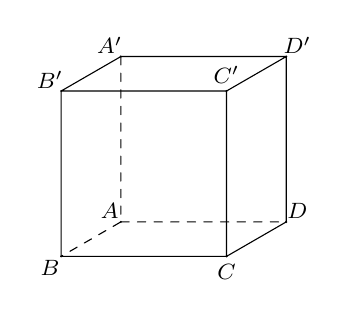
\begin{tikzpicture}[>=stealth,line join=round,line cap=round,font=\footnotesize,scale=0.35]
				\def\r{-150}
				\def\c{6}
				\def\d{2.5}
				\path
				(0:0) coordinate (A)++(0:\c)
				coordinate (D)++(90:\c)coordinate(D')
				(A)++(\r:\d) coordinate (B)++(0:\c) coordinate (C)++(90:\c)coordinate(C')
				(A)++(90:\c) coordinate (A')++(\r:\d) coordinate (B')
				;
				\draw (A')--(B')--(B)--(C)--(D)--(D')--(A') (C)--(C') (B')--(C')--(D');
				\draw[dashed] (A')--(A)--(B) (A)--(D);
				\foreach\p /\r in {A/135,B/-135,D/45,A'/135,B'/135,D'/45,C/-90,C'/90}
				\fill (\p) circle (1.2pt) node[shift={(\r:2mm)}]{$\p$};
	\end{tikzpicture}}}
\end{ex}
%%%=============================%%%

%%%=============EX_14=============%%%
\begin{ex}[Trích đề HKII - THPT Đan Phượng - Hà Nội - NH24-25] 
	\immini[thm]{Cho hình chóp $S. ABCD$ với đáy là hình vuông cạnh $4a$, $SA \perp (ABCD)$, góc giữa $SC$ và mặt đáy là $60^\circ$. Gọi $M$ là trung điểm của đoạn thẳng $BC$, $N$ thuộc $AD$ sao cho $AN = 3a$. Khoảng cách giữa $SB$ và $MN$ bằng
		\choice
		{$\dfrac{8\sqrt{613}}{103}a$}
		{$\dfrac{8\sqrt{629}}{103}a$}
		{$\dfrac{8\sqrt{657}}{103}a$}
		{\True $\dfrac{8\sqrt{618}}{103}a$}
	}{
		\begin{tikzpicture}[scale=.8,line join=round,font=\footnotesize,line cap=round,>=stealth]
			\path
			coordinate (A) at (0,0)
			coordinate (B) at (-1,-1.5)
			coordinate (C) at (3,-1.5)
			coordinate (D) at ($(A)+(C)-(B)$)
			coordinate (S) at ($(A)+(0,3)$)
			;
			\foreach \x/\y/\v in {A/$A$/150,B/$B$/-150,C/$C$/-30,D/$D$/-30,S/$S$/90}{
				\fill (\x) circle (1pt);
				\node at ($(\x)+(\v:3mm)$){\y};}
			\draw (S)--(B)--(C)--(D)--(S)--(C);
			\draw [dashed] (S)--(A)--(B) (A)--(D);
			\draw pic[draw, angle radius=2mm,angle eccentricity=0.3]{right angle=B--A--D};
			\draw pic[draw, angle radius=2mm,angle eccentricity=0.3]{right angle=S--A--D};
			\draw pic[draw, angle radius=2mm,angle eccentricity=0.3]{right angle=S--A--B};
	\end{tikzpicture}}
	\loigiai{
		\begin{center}
			\begin{tikzpicture}[scale=1,line join=round,font=\footnotesize,line cap=round,>=stealth ]
				\path
				coordinate (A) at (0,0)
				coordinate (B) at (-1,-2)
				coordinate (C) at (4,-2)
				coordinate (D) at ($(A)+(C)-(B)$)
				coordinate (S) at ($(A)+(0,4)$)
				coordinate (M) at ($(B)!.5!(C)$)
				coordinate (N) at ($(A)!.75!(D)$)
				coordinate (P) at ($(A)!.25!(D)$)
				coordinate (K) at ($(B)!.9!(P)$)
				coordinate (H) at ($(S)!.9!(K)$);
				\foreach \x/\y/\v in {A/$A$/150,B/$B$/-150,C/$C$/-30,D/$D$/-30,S/$S$/90,M/$M$/-90,N/$N$/60,P/$P$/60,K/$K$/-30,H/$H$/150}{
					\fill (\x) circle (1pt);
					\node at ($(\x)+(\v:3mm)$){\y};}
				\draw (S)--(B)--(C)--(D)--(S)--(C);
				\draw [dashed]
				(S)--(A)--(B)
				(C)--(A)--(D)
				(M)--(N)
				(S)--(P)--(B)
				(H)--(A)--(K)--(S);
				\draw pic[draw,angle radius=2mm] {right angle=B--A--D};
				\draw pic["$60^\circ$",draw,angle radius=4mm,angle eccentricity=2.5] {angle=S--C--A};
				\draw pic[draw,angle radius=1.5mm] {right angle=K--H--A};
				\draw pic[draw,angle radius=1.5mm] {right angle=A--K--B};
			\end{tikzpicture}
		\end{center}
		Ta có hình chiếu của $SC$ trên $(ABCD)$ là $AC$ nên $(SC,(ABCD))=\widehat{SCA}$, suy ra $\widehat{SCA}=60^\circ$.\\
		Do $ABCD$ là hình vuông cạnh $4a$ nên $AC=4\sqrt{2}a$.\\
		Tam giác $SAC$ vuông tại $A$ có $AC=4\sqrt{2}a$, $\widehat{SCA}=60^\circ$ nên
		\[SA=AC=4\sqrt{2}a\cdot \tan60^\circ=4\sqrt{6}a.
		\]
		Gọi $P$ là điểm nằm trên $AD$ sao cho $AP=a$. Khi đó $MN\parallel BP$ và $PN=2PA$, suy ra
		\[\mathrm{d}(NM,SB)=\mathrm{d}(N,(SBP))=2\mathrm{d}(A,(SBP))\quad (1).
		\]
		Gọi $K$, $H$ lần lượt là hình chiếu vuông góc của $A$ lên $BP$ và $SK$ thì $AH\perp(SBP)$, suy ra $\mathrm{d}(A,(SBP))=AH$ \quad ($2$).\\
		Xét hai tam giác vuông $ABP$ có đường cao $AK$ và $SAK$ có đường cao $AH$, ta có
		\[\dfrac{1}{AH^2}=\dfrac{1}{SA^2}+\dfrac{1}{AB^2}+\dfrac{1}{AP^2}=\dfrac{1}{\left(4\sqrt{6}a\right)^2}+\dfrac{1}{(4a)^2}+\dfrac{1}{a^2}=\dfrac{103}{96a^2}\Rightarrow AH=\dfrac{4\sqrt{618}}{103}a\quad (3).\]
		Từ ($1$), ($2$) và ($3$) ta có $\mathrm{d}(NM,SB)=\dfrac{8\sqrt{618}}{103}a$.
	}
\end{ex}
%%%=============================%%%

%%%=============EX_15=============%%%
\begin{ex}
	Cho hình chóp $S. ABC$ có đáy $ABC$ là tam giác đều cạnh $a$. Cạnh bên $SA=a\sqrt{3}$ và vuông góc với mặt đáy $(ABC)$. Tính khoảng cách từ điểm $A$ đến mặt phẳng $(SBC)$.
	\choice
	{\True $\dfrac{a\sqrt{15}}{5}$}
	{$a$}
	{$\dfrac{a\sqrt{5}}{5}$}
	{$\dfrac{a\sqrt{3}}{2}$}
	\loigiai{
		\begin{center}
			\begin{tikzpicture}[scale=0.7, font=\footnotesize, line join=round, line cap=round, >=stealth]
				\def\ac{4} % cạnh AC
				\def\ba{2} % cạnh BA
				\def\h{3.5} % đường cao
				\def\gocA{-45} % góc A của đáy
				\coordinate[label=left:$A$] (A) at (0,0);
				\coordinate[label=below:$B$] (B) at (\gocA:\ba);
				\coordinate[label=right:$C$] (C) at (\ac,0);
				\coordinate[label=above:$S$] (S) at ($(A)+(90:\h)$);
				\coordinate[label=below right:$E$] (E) at ($(B)!0.5!(C)$);
				\coordinate[label=right:$F$] (F) at ($(S)!(A)!(E)$);
				\draw (S)--(A)--(B)--(C)--cycle (S)--(B) (S)--(E);
				\draw[dashed] (E)--(A) (A)--(C) (A)--(F);
				\foreach \diem in {A,B,C,S,E,F}	\fill (\diem)circle(1.2pt);
				\path 
				pic[draw,angle radius=5]{right angle=A--F--S} 
				pic[draw,angle radius=5]{right angle=A--E--B};
				
			\end{tikzpicture}
		\end{center}
		Trong mặt phẳng $(ABC)$, gọi $E$ là trung điểm của $BC$.\\
		Vì $\triangle ABC$ là tam giác đều cạnh $a$ nên $AE \perp BC$ và $AE = \dfrac{a\sqrt{3}}{2}$.\\
		Ta có
		$\heva{ & BC \perp AE \\ & BC \perp SA \quad (\text{do } SA \perp (ABC)) } \Rightarrow BC \perp (SAE)$.\\
		Trong mặt phẳng $(SAE)$, kẻ $AF \perp SE$ tại $F$.\\
		Vì $BC \perp (SAE)$ nên $BC \perp AF$.\\
		Ta có
		$\heva{ & AF \perp SE \\ & AF \perp BC } \Rightarrow AF \perp (SBC)$.\\
		Do đó, khoảng cách từ $A$ đến mặt phẳng $(SBC)$ là $\mathrm{d}\big(A,(SBC)\big) = AF$.\\
		Xét tam giác $SAE$ vuông tại $A$, có đường cao $AF$, ta có
		\[ \dfrac{1}{AF^2} = \dfrac{1}{SA^2} + \dfrac{1}{AE^2} = \dfrac{1}{(a\sqrt{3})^2} + \dfrac{1}{\left(\dfrac{a\sqrt{3}}{2}\right)^2} = \dfrac{1}{3a^2} + \dfrac{4}{3a^2} = \dfrac{5}{3a^2}. \]
		Suy ra $AF^2 = \dfrac{3a^2}{5}$, do đó $AF = \dfrac{a\sqrt{15}}{5}$.\\
		Vậy $\mathrm{d} = \dfrac{a\sqrt{15}}{5}$.
	}
\end{ex}
%%%=============================%%%

%%%=============EX_16=============%%%
\begin{ex}
	Cho hình chóp $S. ABC$ có đáy $ABC$ là tam giác vuông tại $B$, với $BA=BC=a$, $SA=a$ và $SA$ vuông góc với đáy. Khoảng cách từ $A$ tới mặt phẳng $(SBC)$ là
	\choice
	{$\dfrac{\sqrt{2}}{3}a$}
	{$\dfrac{1}{2}a$}
	{$\dfrac{\sqrt{3}}{2}a$}
	{\True $\dfrac{a\sqrt{2}}{2}$}
	\loigiai{
		\immini{
			Ta có $SA \perp (ABC)$ nên $SA \perp BC$.\\
			Lại có $AB \perp BC$ (do $\triangle ABC$ vuông tại $B$).\\
			Từ đó suy ra $\heva{ & BC \perp SA \\ & BC \perp AB } \Rightarrow BC \perp (SAB)$.\\
			Trong mặt phẳng $(SAB)$, kẻ đường cao $AH \perp SB$ tại $H$.\\
			Vì $BC \perp (SAB)$ nên $BC \perp AH$.\\
			Ta có $\heva{ & AH \perp SB \\ & AH \perp BC } \Rightarrow AH \perp (SBC)$.\\
			Vậy khoảng cách từ $A$ đến mặt phẳng $(SBC)$ là $\mathrm{d}\big(A, (SBC)\big) = AH$.\\
			Xét tam giác $SAB$ vuông tại $A$ (do $SA \perp (ABC)$ nên $SA \perp AB$), có đường cao $AH$. Áp dụng hệ thức lượng, ta có
			\[ \dfrac{1}{AH^2} = \dfrac{1}{SA^2} + \dfrac{1}{AB^2} = \dfrac{1}{a^2} + \dfrac{1}{a^2} = \dfrac{2}{a^2}. \]
			Suy ra $AH^2 = \dfrac{a^2}{2}$, do đó $AH = \dfrac{a\sqrt{2}}{2}$.
		}{
			\begin{tikzpicture}[scale=0.7, font=\footnotesize, line join=round, line cap=round, >=stealth]
				\def\ac{4} % cạnh AC
				\def\ba{2} % cạnh BA
				\def\h{3} % đường cao
				\def\gocA{-45} % góc A của đáy
				\coordinate[label=left:$A$] (A) at (0,0);
				\coordinate[label=below:$B$] (B) at (\gocA:\ba);
				\coordinate[label=right:$C$] (C) at (\ac,0);
				\coordinate[label=above:$S$] (S) at ($(A)+(90:\h)$);
				\coordinate[label=right:H] (H) at ($(S)!(A)!(B)$);
				\draw (S)--(A)--(B)--(C)--cycle (S)--(B) (A)--(H);
				\draw[dashed] (A)--(C);
				\foreach \diem in {A,B,C,S,H}	\fill (\diem)circle(1.2pt); 
				\path 
				pic[draw,angle radius=5]{right angle=A--H--S};
			\end{tikzpicture}	
		}
		
	}
\end{ex}
%%%=============================%%%

%%%=============EX_17=============%%%
\begin{ex}
	Cho hình hộp chữ nhật $ABCD. A'B'C'D'$ có $\,AA'=5a.$ Tính khoảng cách giữa đường thẳng $AC$ và $\left(A'B'C'D'\right)$ .
	\choice
	{$\sqrt{34}a$}
	{$\sqrt{41}a$}
	{$8a$}
	{\True $5a$}
	\loigiai{ 
		\immini{Ta có $\left\{\begin{array}{l}
				AC \parallel A'C'\\
				A'C'\subset\left(A'B'C'D'\right),AC\not\subset\left(A'B'C'D'\right)
			\end{array}\right.\Rightarrow AC \parallel \left(A'B'C'D'\right).$\\
			Do đó, $\mathrm{d}\left(AC,\left(A'B'C'D'\right)\right)=\mathrm{d}\left(A,\left(A'B'C'D'\right)\right).$\\
			Mà $ABCD. A'B'C'D'$ là hình hộp chữ nhật nên \[\mathrm{d}\left(A,\left(A'B'C'D'\right)\right)=AA'=5a.\]
			Vậy $d\left(AC,\left(A'B'C'D'\right)\right)=5a$. }{
			\begin{tikzpicture}[scale=0.7, font=\footnotesize, line join=round, line cap=round, >=stealth]
				\def\bc{4} % cạnh BC
				\def\ba{2} % cạnh BA
				\def\h{3} % đường cao
				\def\gocB{45} % góc B của đáy
				\coordinate[label=left:$B$] (B) at (0,0);
				\coordinate[label=above:$A$] (A) at (\gocB:\ba);
				\coordinate[label=right:$C$] (C) at (\bc,0);
				\coordinate[label=above:$D$] (D) at ($(A)+(C)-(B)$);
				\coordinate[label=left:$A'$] (A') at ($(A)+(-90:\h)$);
				\coordinate[label=below:$B'$] (B') at ($(B)+(A')-(A)$);
				\coordinate[label=below:$C'$] (C') at ($(C)+(A')-(A)$);
				\coordinate[label=right:$D'$] (D') at ($(D)+(A')-(A)$);
				\draw (A)--(B)--(B')--(C')--(D')--(D)--cycle (C)--(C') (B)--(C)--(D) (A)--(C);
				\draw[dashed] (A)--(A')node[right,pos=0.65]{$ 5a $} (B')--(A')--(D') (A')--(C');
				\foreach \diem in {A,B,C,D,A',B',C',D'}	\fill (\diem)circle(1.2pt);
		\end{tikzpicture}}
	}
\end{ex}
%%%=============================%%%

%%%=============EX_18=============%%%
\begin{ex}
	Cho hình chóp tam giác đều $S. ABC$ có cạnh đáy bằng $\;3a,$ cạnh bên bằng $2a$ . Gọi $ M,N,P$ lần lượt là trung điểm của $ SA,SB,SC.$ Tính khoảng cách giữa hai mặt phẳng $\left(MNP\right)$ và $\left(ABC\right)$ .
	\choice
	{$4a$}
	{$3a$}
	{$2a$}
	{\True $\dfrac{a}{2}$}
	\loigiai{
		\immini{Gọi $SH$ là đường cao của hình chóp $S. ABC$, giả sử $D=SH\cap\left(MNP\right)$.\\
			Ta có $\left(MNP\right)\parallel\left(ABC\right)$ nên \[\mathrm{d}\left(\left(MNP\right);\left(ABC\right)\right)=\mathrm{d}\left(D;\left(ABC\right)\right)=DH.\]
			Tam giác $ABC$ đều cạnh $3a$ nên \[AH=\dfrac{2}{3}\cdot 3a \cdot \dfrac{\sqrt{3}}{2}=a\sqrt{3}.\]
			Do đó $SH=\sqrt{SA^2-AH^2}=\sqrt{4a^2-3a^2}=a$.\\
			Từ đó suy ra $DH=\dfrac{1}{2}\cdot SH=\dfrac{a}{2}$.\\
			Vậy $\mathrm{d}\left(\left(MNP\right);\left(ABC\right)\right)=\dfrac{a}{2}.$}{
			 \begin{tikzpicture}[scale=1, font=\footnotesize, line join=round, line cap=round, >=stealth] 
				\def\ba{5} % cạnh BA
				\def\bc{2} % cạnh BC
				\def\h{4} % đường cao
				\def\gocB{-60} % góc B của đáy
				\coordinate[label=left:$B$] (B) at (0,0);
				\coordinate[label=below:$C$] (C) at (\gocB:\bc);
				\coordinate[label=right:$A$] (A) at (\ba,0);
				\coordinate[label=above left:$$] (I) at ($(A)!1/2!(C)$);
				\coordinate[label=below:$H$] (H) at ($(B)!0.5!(I)$);
				\coordinate[label=above:$S$] (S) at ($(H)+(90:\h)$);
				\coordinate[label=right:M] (M) at ($(S)!.5!(A)$);
				\coordinate[label=left:N] (N) at ($(S)!.5!(B)$);
				\coordinate[label= left:P] (P) at ($(S)!.5!(C)$);
				\coordinate[label=right:D] (D) at ($(S)!.5!(H)$);
				\draw (S)--(A)--(B)--(C)--(A)--(S)--(C)--(B)--(S) (M)--(N)--(P)--cycle ;
				\draw[dashed] (S)--(H) ; 
				\foreach \diem in {A,B,C,S,N,H,M,P,D}	\fill (\diem)circle(1.2pt);
				
		\end{tikzpicture}
	}
	}
\end{ex}
%%%=============================%%%

%%%=============EX_19=============%%%
\begin{ex}
	Cho hình chóp $ S. ABCD$ có $ABCD$ là hình thang vuông ở $A$ và $D$ , $AD=2a.$ $SD\perp\left(ABCD\right)$ và $SD=a\sqrt 2 $. Tính khoảng cách giữa đường thẳng $DC$ và $\left(SAB\right)$.
	\choice
	{$a\sqrt 2 $}
	{$\dfrac{a\sqrt 3}{3}$}
	{$\dfrac{a}{\sqrt 2}$}
	{\True $\dfrac{2a}{\sqrt 3}$}
	\loigiai{ \immini{ Ta có $ DC\parallel\left(SAB\right)$ nên $ \mathrm{d}\left(DC,\left(SAB\right)\right)=\mathrm{d}\left(D,\left(SAB\right)\right)$.\\
			Dựng $ DK\perp SA$, do $\left\{\begin{array}{l}
				AB\perp SD\\
				AB\perp AD
			\end{array}\right.\Rightarrow AB\perp\left(SAD\right)\Rightarrow AB\perp DK$. \\ Từ đó suy ra $ DK\perp\left(SAB\right)$ và $ \mathrm{d}\left(DC,\left(SAB\right)\right)=\mathrm{d}\left(D,\left(SAB\right)\right)=DK$.\\
			Mà $\dfrac{1}{D{K^2}}=\dfrac{1}{S{D^2}}+\dfrac{1}{A{D^2}}=\dfrac{1}{2a^2}+\dfrac{1}{4a^2}=\dfrac{3}{4a^2}$ $\Rightarrow DK=\dfrac{2a}{\sqrt 3}$. \\ Vậy $ \mathrm{d}\left(D,\left(SAB\right)\right)=\dfrac{2a}{\sqrt 3}$. }{
			\begin{tikzpicture}[>=stealth, line join=round, line cap = round,scale=0.8]
				\path
				(0,0) coordinate (D)
				--++(-2,-2) coordinate (A)
				--++(4,0)    coordinate (B)
				--++(4,2)    coordinate (C)
				(D)--++(0,3)    coordinate (S)
				;
				\coordinate[label=above left:] (K) at ($(S)!(D)!(A)$);
				\draw (S)--(B)--(C)--(S)--(A)--(B);
				\draw[dashed] (S)--(D)node[right,pos=0.75]{$ a\sqrt{2} $} (A)--(D)node[right,pos=0.5]{$ 2a $} (D)--(C) (D)--(K);
				\foreach \i/\g in {S/90, A/-80, B/-90, C/-90, D/-90,K/180}
				\fill (\i) circle (1pt)+(\g:3mm) node {$\i$};
				\path 
				pic[draw,angle radius=5]{right angle=D--A--B}
				pic[draw,angle radius=5]{right angle=S--K--D}
				pic[draw,angle radius=5]{right angle=A--D--C}
				pic[draw,angle radius=5]{right angle=S--D--C}
				;
		\end{tikzpicture}}
	}
\end{ex}
%%%=============================%%%

%%%=============EX_20=============%%%
\begin{ex}
	Cho hình chóp $ S. ABC$ có đáy $ ABCD$ là hình vuông cạnh $ a$, tâm $ O$. Cạnh bên $ SA=2a$ và vuông góc với mặt đáy $\left(ABCD\right)$. Gọi $ H$ và $ K$ lần lượt là trung điểm của cạnh $ BC$ và $ CD$. Tính khoảng cách giữa hai đường thẳng $ HK$ và $ SD$.
	\choice
	{\True $\dfrac{a}{3}$}
	{$\dfrac{2a}{3}$}
	{$ 2a$}
	{$\dfrac{a}{2}$}
	\loigiai{ \immini{	Gọi $ E=HK\cap AC.$ Do $ HK \parallel BD$ nên \[ \mathrm{d}\left[HK,SD\right]=\mathrm{d}\left[HK,\left(SBD\right)\right] =\mathrm{d}\left[E,\left(SBD\right)\right]=\dfrac{1}{2}\mathrm{d}\left[A,\left(SBD\right)\right].\]
			Kẻ $AF\perp SO$ . Khi đó \[ \mathrm{d}\left[A,\left(SBD\right)\right]=AF=\dfrac{SA\cdot AO}{\sqrt{S{A^2}+A{O^2}}}=\dfrac{2a}{3}.\]
			Vậy $ \mathrm{d}\left[HK,SD\right]=\dfrac{1}{2}AF=\dfrac{a}{3}.$}{ 
			\begin{tikzpicture}[>=stealth, line join=round, line cap = round,scale=1]
				\path
				(0,0) coordinate (A)
				--++(-1,-2) coordinate (B)
				--++(4,0)    coordinate (C)
				--++(1,2)    coordinate (D)
				(A)--++(0,3)    coordinate (S)
				;
				\path (intersection of A--C and B--D) coordinate[label=above right:] (O);
				\coordinate[label=below:] (F) at ($(S)!(A)!(O)$);
				\coordinate[label=above:] (K) at ($(D)!.5!(C)$);
				\coordinate[label=above:] (H) at ($(B)!.5!(C)$);
				\path (intersection of A--C and H--K) coordinate[label=above right:] (E);
				\draw (S)--(B)--(C)--(D)--(S)--(B) (S)--(C);
				\draw[dashed] (S)--(A)--(B) (D)--(A) (S)--(O) (H)--(K) (A)--(C) (B)--(D) (A)--(F) ; 
				\foreach \i/\g in {S/90, A/-80, B/-90, C/-90, D/0,F/45,H/-90,K/-90,E/-90,O/-90}
				\fill (\i) circle (1pt)+(\g:3mm) node {$\i$};
				\path 
				pic[draw,angle radius=5]{right angle=S--A--B}
				pic[draw,angle radius=5]{right angle=S--A--D}
				pic[draw,angle radius=5]{right angle=A--O--D}
				pic[draw,angle radius=5]{right angle=A--F--S}
				;
		\end{tikzpicture} }
	}
\end{ex}
%%%=============================%%%
\Closesolutionfile{ans}
\ind{PHẦN II.} \inden{Câu trắc nghiệm đúng sai. Trong mỗi ý a), b), c), d) ở mỗi câu, học sinh chọn đúng hoặc sai.}\\
\setcounter{ex}{0}
\Opensolutionfile{ans}[ans/1H8-Bai4-DS]
%%%=============EX_1=============%%%
\begin{ex}[Trích đề HKII - THPT Lê Quý Đôn - Bắc Ninh - NH24-25] 
	Cho hình chóp $S. ABC$ có hai mặt phẳng $(SAB)$ và $(SAC)$ cùng vuông góc với đáy. Tam giác $ABC$ vuông cân tại $B$, $BC = a$. Góc giữa đường thẳng $SB$ và mặt phẳng $(ABC)$ bằng $60^\circ$.
	\choiceTF
	{$\mathrm{d}(A, (SBC)) = \dfrac{a\sqrt{3}}{3}$}
	{\True $BC \perp (SAB)$}
	{\True $SA \perp (ABC)$}
	{$SA = a$}
	\loigiai{
		\begin{center}
			\begin{tikzpicture}[font=\footnotesize, line join=round, line cap=round,scale=.7, >=stealth]
				\path (0,0) coordinate (A)(4,0) coordinate (C)
				(1.5,-1.5) coordinate (B)
				($(A)+(90:3)$) coordinate (S)
				($(S)!0.5!(B)$) coordinate (H)
				;
				\draw (H)--(A)--(B)--(C)
				(A)--(S)(B)--(S)(C)--(S)--(B);
				\draw[dashed] (A)--(C);
				\pic[draw,angle radius=1.5mm,angle eccentricity=1.5] {right angle = S--A--B};
				\pic[draw,angle radius=1.5mm,angle eccentricity=1.5] {right angle = A--H--B};
				\pic[draw,angle radius=1.5mm,angle eccentricity=1.5] {right angle = A--B--C};
				\pic[draw,angle radius=1.5mm,angle eccentricity=1.5] {right angle = S--A--C};
				\draw pic[draw,angle radius=15,angle eccentricity=1.5]{angle=S--B--A};
				\foreach \x /\goc in {A/180,C/0,B/-135,S/90,H/50}
				\fill[black] (\x) circle (1pt)
				($(\x)+(\goc:3mm)$) node {$\x$};
			\end{tikzpicture}
		\end{center}
		\begin{itemchoice}
			\itemch 
			Trong mặt phẳng $(SAB)$, kẻ đường cao $AH \perp SB$ tại $H$.\\
			Ta có $BC \perp (SAB)$, suy ra $BC \perp AH$.\\
			Vì $AH$ vuông góc với cả $SB$ và $BC$, nên $AH \perp (SBC)$.\\
			Do đó, khoảng cách từ $A$ đến mặt phẳng $(SBC)$ là $$\mathrm{d}(A, (SBC)) = AH=\dfrac{SA\cdot AB}{\sqrt{SA^2+AB^2}}=\dfrac{a\sqrt{3}\cdot a}{\sqrt{(a\sqrt{3})^2+a^2}}=\dfrac{a\sqrt{3}}{2}.$$
			\itemch 
			Ta có $\heva{
				& BC \perp AB \text{ (do } \triangle ABC \text{ vuông cân tại } B)\\
				& BC \perp SA, \text{ (do } SA \perp (ABC))\\
				& AB, SA \subset (SAB) \text{ và } AB \cap SA = \{A\}}\Rightarrow BC \perp (SAB)$.
			\itemch 
			Ta có
			$\heva{
				& (SAB) \perp (ABC) \\
				& (SAC) \perp (ABC) \\
				& (SAB) \cap (SAC) = SA} \Rightarrow SA \perp (ABC)$.
			\itemch 
			Vì $SA \perp (ABC)$ nên hình chiếu của $SB$ lên mặt phẳng $(ABC)$ là $AB$.\\
			Do đó, góc giữa đường thẳng $SB$ và mặt phẳng $(ABC)$ là góc $\widehat{SBA}$. Theo giả thiết, $\widehat{SBA} = 60^\circ$.\\
			Xét tam giác $\triangle SAB$ vuông tại $A$ ta có $\tan\widehat{SBA} = \dfrac{SA}{AB}$.\\
			Vì $\triangle ABC$ vuông cân tại $B$ có $BC=a$, suy ra $AB = BC = a$.\\
			Ta có $\tan60^\circ = \dfrac{SA}{a} \Rightarrow SA = a \cdot \tan60^\circ = a\sqrt{3}$.
		\end{itemchoice}
	}
\end{ex}
%%%=============================%%%

%%%=============EX_2=============%%%
\begin{ex}[Trích đề HKII - THPT Chuyên Lê Quý Đôn - Ninh Thuận - NH24-25] 
	Cho hình chóp $S. ABCD$ có đáy $ABCD$ là hình vuông tâm $O$ cạnh $2a$, tam giác $SAD$ cân tại $S$ có $SA=SD=a\sqrt{13}$. Hình chiếu của $S$ lên mặt phẳng $\left(ABCD\right)$ trùng với trung điểm $H$ của cạnh $AD$.
	\begin{center}
		\begin{tikzpicture}[scale=.7,line join=round,line cap=round,font=\footnotesize,>=stealth]
			\def\a{4}
			\def\h{4.5}
			\path (0:0) coordinate (A)
			++(0:\a) coordinate (B)
			++(-130:\a/2) coordinate (C)
			($(A)+(C)-(B)$) coordinate (D)
			($(A)!0.5!(D)$) coordinate (H)
			($(H)+(90:\h)$) coordinate (S)
			(intersection of A--C and B--D) coordinate (O);%giao điểm O
			\draw[dashed,thick] (D)--(A)--(B)(A)--(S)
			(S)--(H)(A)--(C) (B)--(D) ;
			\draw[thick] (D)--(C)--(B)
			(B)--(S)(C)--(S)(D)--(S) ;
			\foreach \x/\g in {A/135,D/-135,C/-45,B/45,S/90,H/135,O/-90}
			\fill[black] (\x) circle (1.5pt)
			($(\g:4mm)+(\x)$) node {$\x$};
		\end{tikzpicture}
	\end{center}
	\choiceTF
	{\True $\left(SAD\right)\perp\left(SAB\right)$}
	{\True Gọi $E$ là trung điểm đoạn thẳng $HO$ . Khoảng cách từ $E$ đến mặt phẳng $\left(SBC\right)$ bằng $\dfrac{3a\sqrt 3}{4}$}
	{Số đo góc nhị diện $\left[S,BC,H\right]$ bằng $30^\circ $}
	{\True $SH\perp\left(ABCD\right)$}
	\loigiai{
		\begin{center}
			\begin{tikzpicture}[scale=.7,line join=round,line cap=round,font=\footnotesize,>=stealth]
				\def\a{4}
				\def\h{4.5}
				\path (0:0) coordinate (A)
				++(0:\a) coordinate (B)
				++(-130:\a/2) coordinate (C)
				($(A)+(C)-(B)$) coordinate (D)
				($(A)!0.5!(D)$) coordinate (H)
				($(H)+(90:\h)$) coordinate (S)
				(intersection of A--C and B--D) coordinate (O)
				($(H)!0.5!(O)$) coordinate (E)
				($(B)!0.5!(C)$) coordinate (I)
				($(S)!0.6!(I)$) coordinate (K);%giao điểm O
				\draw[dashed,thick] (D)--(A)--(B)(A)--(S)
				(S)--(H)(A)--(C) (B)--(D) (H)--(I) (H)--(K);
				\draw[thick] (D)--(C)--(B)
				(B)--(S)(C)--(S)(D)--(S) (S)--(I);
				\foreach \x/\g in {A/135,D/-135,C/-45,B/45,S/90,H/135,O/-90,E/-145,I/0,K/0}
				\fill[black] (\x) circle (1.5pt)
				($(\g:4mm)+(\x)$) node {$\x$};
				\draw pic[draw,angle radius=3mm]{right angle=H--K--S};%Theo chiều dương
			\end{tikzpicture}
		\end{center}
		\begin{itemchoice}
			\itemch Ta có $AB \perp AD$ ($ABCD$ là hình vuông), $AB \perp SH$ vì $SH \perp (ABCD)$.\\ Suy ra $AB \perp (SAD) \Rightarrow (SAD) \perp (SAB)$.
			\itemch Gọi $K$ là chân đường cao kẻ từ $H$ của tam giác $SHI$.\\
			Ta có $HK \perp SI$ và $HK \perp BC$, suy ra $HK \perp (SBC)$.\\
			Khi đó $\mathrm{d}(H,(SBC))=HK$.\\
			Xét tam giác $SHI$ vuông tại $H$, ta có\\
			$\dfrac{1}{HK^2}=\dfrac{1}{SH^2}+\dfrac{1}{HI^2}=\dfrac{1}{12a^2}+\dfrac{1}{4a^2}=\dfrac{1}{3a^2}\Rightarrow HK=\sqrt{3}a$.\\
			Vì $E$ là trung điểm của $HO$ nên $EI=\dfrac{3}{4}HI$.\\ Suy ra
			$\mathrm{d}(E,(ABC))=\dfrac{3}{4}\mathrm{d}(H,(SBC))=\dfrac{3}{4}\sqrt{3}a=\dfrac{3\sqrt{3}a}{4}$.
			\itemch Gọi $I$ là trung điểm đoạn thẳng $BC$.\\
			Khi đó
			$SI \perp BC$, $HI \perp BC \Rightarrow [S,BC,H]=\widehat{SIH}$.\\
			Tam giác $SAH$ vuông tại $H$ có $SA=a\sqrt{13}$, $AH=a$.\\
			Suy ra $SH=\sqrt{SA^2-AH^2}=\sqrt{13a^2-a^2}=2\sqrt{3}a$.\\
			Xét tam giác $SHI$ vuông tại $H$, ta có
			$\tan (SIH)=\dfrac{SH}{HI}=\dfrac{2\sqrt{3}a}{2a}=\sqrt{3}$.\\
			Suy ra $[S,BC,H]=\widehat{SIH}=60^\circ$.
			\itemch Ta có hình chiếu của $S$ lên mặt phẳng $\left(ABCD\right)$ trùng với trung điểm $H$ của cạnh $AD$, suy ra $SH\perp\left(ABCD\right)$.
		\end{itemchoice}
	}
\end{ex}
%%%=============================%%%

%%%=============EX_3=============%%%
\begin{ex}[Trích đề HKII - THPT Lý Thái Tổ - Bắc Ninh - NH24-25]
	Cho hình chóp $S. ABCD$ có đáy $ABCD$ là hình chữ nhật với $AB=4$ và $AD=2$. Mặt bên $(SAB)$ là tam giác đều và vuông góc với mặt đáy. Gọi $H$, $K$ lần lượt là trung điểm các cạnh $AB$ và $CD$.
	\choiceTF
	{\True Hai mặt phẳng $(SHC)$ và $(SKB)$ vuông góc}
	{\True Đường thẳng $SH$ vuông góc mặt phẳng $(ABCD)$}
	{Cosin góc giữa đường thẳng $SD$ và mặt đáy bằng $\dfrac{\sqrt{15}}{5}$}
	{\True Khoảng cách giữa đường thẳng $AB$ và mặt phẳng $(SCD)$ bằng $\sqrt{3}$}
	\loigiai
	{ \begin{center}
			\begin{tikzpicture}[scale=0.7, font=\footnotesize,line join=round, line cap=round, >=stealth]
				\path
				(0,0) coordinate (A)
				++(-140:2) coordinate (B)
				++(0:4) coordinate (C)
				($(A)+(C)-(B)$) coordinate (D)
				($(A)!1/2!(B)$) coordinate (H)
				($(H)+(0,4)$) coordinate (S)
				($(C)!1/2!(D)$) coordinate (K)
				($(S)!(H)!(K)$) coordinate (M)
				;
				\foreach \i in{B,C,D}{\draw (S)--(\i);};
				\draw (B)--(C)--(D) (S)--(K);
				\draw[dashed] (S)--(A)--(B) (A)--(D) (S)--(H)--(K) (H)--(M);
				\pic[draw,angle eccentricity=1.8,angle radius=2mm]{right angle=S--H--A};
				\foreach \i/\g in {A/-90,B/-90,C/-90,D/-90,S/90,H/-60,K/-90,M/0}
				\fill[black] (\i) circle(1pt)+(\g:3mm)node[scale=1]{$\i$};
			\end{tikzpicture}
		\end{center}
		\begin{itemchoice}
			\itemch Ta có $\heva{&BK\perp HC\quad (HKCB \text{ là hình vuông})\\ & BK\perp SH \\& BK\subset(SBK)}\Rightarrow (SHC)\perp (SKB)$.
			\itemch Ta có $\heva{& SH \subset (SAB),SH\perp AB \\ & (SAB)\perp (ABCD)\\& (SAB)\cap(ABCD)=AB}\Rightarrow SH\perp (ABCD)$.
			\itemch Ta có $SH\perp(ABCD)$ nên góc giữa $SD$ và $(ABCD)$ là góc giữa $SD$ và $HD$.\\
			Trong tam giác vuông $SHD$ có $\tan \widehat{SDH}=\dfrac{SH}{HD}=\dfrac{2\sqrt{3}}{2\sqrt{2}}=\dfrac{\sqrt{3}}{\sqrt{2}}$.\\
			Suy ra $\cos \widehat{SDH}=\sqrt{\dfrac{1}{1+\tan^2\widehat{SDH}}}=\sqrt{\dfrac{1}{1+\dfrac{3}{2}}}=\dfrac{\sqrt{10}}{5}$.
			\itemch
			Trong $(SHK)$, vẽ $HM\perp SK, M\in SK$.\\
			Khi đó $\mathrm{d}(A,(SCD))=\mathrm{d}(H,(SCD))=HM$.\\
			Ta có $\dfrac{1}{HM^2}=\dfrac{1}{SH^2}+\dfrac{1}{HK^2}\Rightarrow HM=\sqrt{\dfrac{SH^2\cdot HK^2}{SH^2+ HK^2}}=\sqrt{\dfrac{12\cdot4}{16}}= \sqrt{3}$.\\
			Vậy $\mathrm{d}(A,(SCD))=\sqrt{3}$.
		\end{itemchoice}
	}
\end{ex}
%%%=============================%%%

%%%=============EX_4=============%%%
\begin{ex}[Trích đề HKII - THPT Việt Nam - Ba Lan - Hà Nội - NH24-25] 
	Cho hình lập phương $ABCD. A'B'C'D'$ có cạnh bằng $2\sqrt{3}$.
	\choiceTF
	{Khoảng cách giữa hai mặt phẳng $\left(D'AC\right)$, $\left(BC'A'\right)$ bằng $\dfrac{2\sqrt{6}}{3}$}
	{\True Mặt phẳng $\left(D'AC\right)$ vuông góc với mặt phẳng $\left(BDD'B'\right)$}
	{\True Gọi $O$ là tâm của hình vuông $ABCD$. Giao điểm của đường thẳng $DB'$ và mặt phẳng $\left(D'AC\right)$ là giao điểm của hai đường thẳng $DB'$ và $D'O$}
	{Độ dài đường chéo của hình lập phương bằng $2\sqrt{6}$}
	
	\loigiai{
		\begin{center}
			\begin{tikzpicture}[scale=1, font=\footnotesize, line join=round, line cap=round, >=stealth]
				\coordinate (A) at (0,0);
				\coordinate (D) at (3,0);
				\coordinate (B) at (-1,-0.5);
				\coordinate (C) at ($(B)+(3,0)$);
				\foreach \x in {A,B,C,D}{
					\coordinate (\x') at ($(\x)+(0,3)$);
				}
				\coordinate (O) at ($(A)!0.5!(C)$);
				\coordinate (O') at ($(A')!0.5!(C')$);
				\coordinate (H) at ($(O)!0.4!(D')$);
				\draw (B')--(A')--(D')--(C')--(B')--(B)--(C)--(D)--(D')--(C)--(C') (A')--(C');
				\draw[dashed] (A')--(A)--(B) (A)--(D)--(B) (D)--(B') (C)--(A)--(D') (D')--(O) (B)--(O') (D)--(H);
				\foreach \x/\y in {A/135,B/180,C/-90,D/0,A'/90,B'/180,C'/90,D'/0,O/20,O'/20,H/160}{
					\draw[fill=black] (\x) circle (1pt) ($(\x)+(\y:3mm)$) node {$\x$};
				}
			\end{tikzpicture}
		\end{center}
		\begin{itemchoice}
			\itemch Ta có $\heva{&A'C'\parallel AC\\&BO'\parallel D'O\\&A'C',BO' \subset \left(BC'A'\right)\\&AC,D'O \subset \left(D'AC\right)}\Rightarrow \left(D'AC\right)\parallel \left(BC'A'\right)\\
			\Rightarrow \mathrm{d}\left(\left(D'AC\right),\left(BC'A'\right)\right)=\mathrm{d}\left(B,\left(D'AC\right)\right)$.\\
			Mà $\dfrac{\mathrm{d}\left(B,\left(D'AC\right)\right)}{\mathrm{d}\left(D,\left(D'AC\right)\right)}=\dfrac{BO}{DO}=1\Rightarrow \mathrm{d}\left(B,\left(D'AC\right)\right)=\mathrm{d}\left(D,\left(D'AC\right)\right)$.\\
			Vẽ $DH\perp D'O$ tại $H$.\\
			Ta có $\heva{&AC\perp OD\\&AC\perp DD'\\&OD,DD' \subset \left(ODD'\right)}\Rightarrow AC\perp \left(ODD'\right)\Rightarrow AC\perp DH$.\\
			Mà $\heva{&DH\perp D'O\\&D'O,AC \subset \left(D'AC\right)}\Rightarrow DH\perp \left(D'AC\right)$.\\
			Suy ra $\mathrm{d}\left(D,\left(D'AC\right)\right)=DH$.\\
			$OD=2\sqrt{3}\cdot \dfrac{\sqrt{2}}{2}=\sqrt{6}$.\\
			$D'O=\sqrt{OD^2+DD'^2}=\sqrt{\left(\sqrt{6}\right)^2+\left(2\sqrt{3}\right)^2}=3\sqrt{2}$.\\
			$DH=\dfrac{OD\cdot DD'}{D'O}=\dfrac{\sqrt{6}\cdot 2\sqrt{3}}{3\sqrt{2}}=2$.
			\itemch Ta có $AC\perp BD$, $AC\perp AA' \Rightarrow AC\perp \left(BDD'B'\right)$.\\
			Mà $AC \subset \left(D'AC\right) \Rightarrow \left(D'AC\right)\perp \left(BDD'B'\right)$.
			\itemch Ta có $D'O$, $DB'\subset \left(BDD'B'\right)\Rightarrow D'O \cap DB'$.\\
			Mà $D'O \subset \left(D'AC\right)$ nên giao điểm của đường thẳng $DB'$ và mặt phẳng $\left(D'AC\right)$ là giao điểm của hai đường thẳng $DB'$ và $D'O$.
			\itemch $AC'=2\sqrt{3}\cdot\sqrt{3}=6$.
		\end{itemchoice}
	}
\end{ex}
%%%=============================%%%

%%%=============EX_5=============%%%
\begin{ex}[Trích đề HKII - THPT Chuyên Trần Đại Nghĩa - TP Hồ Chí Minh - NH24-25]
	Cho hình chóp đều $S. ABCD$ có $O$ là tâm của hình vuông $ABCD$, $SA = 2a$, $AB = a$. Gọi $H$ là trực tâm của $\triangle SBC$ (tham khảo hình vẽ).
	\begin{center}
		\begin{tikzpicture}[scale=0.6, font=\footnotesize, line join=round, line cap=round, >=stealth]
			\path (0,0)coordinate(A)
			--++(-2,-2) coordinate(D)
			--++(5,0) coordinate(C)
			(A)--+(5,0) coordinate (B)
			(A)--(C)coordinate[pos=0.5](O)
			(O)--+(0,5) coordinate (S)
			(B)--(C)coordinate[pos=0.5](M)
			(S)--(M)coordinate[pos=0.7](H)
			;
			\draw (S)--(D)--(C)--(B)--cycle (S)--(C) (S)--(M);
			\draw[dashed] (O)--(S)--(A) (A)--(D) (A)--(B) (A)--(C) (D)--(B);
			\draw pic[draw, angle radius=0.2cm]{right angle=S--O--C};
			\draw pic[draw, angle radius=0.2cm]{right angle=S--O--D};
			\foreach \p/\q in {A/40,D/-90,C/-90,B/40,S/90,O/-90,H/30}{
				\path (\p) node[shift={(\q:3mm)}]{$\p$};
				\fill[black] (\p) circle (1.2pt);}
		\end{tikzpicture}
	\end{center}
	Trong các khẳng định sau, khẳng định nào đúng?
	\choiceTF
	{\True $\mathrm{d}(AB, (SCD)) = \dfrac{\sqrt{210}}{15}a$}
	{$(BD, SA) = 60^\circ$}
	{$V_{S. ABCD} = SO \cdot S_{ABCD}$}
	{\True $(SBC) \perp (SOH)$}
	\loigiai{
		\begin{center}
			\begin{tikzpicture}[scale=0.6, font=\footnotesize, line join=round, line cap=round, >=stealth]
				\path (0,0)coordinate(A)
				--++(-2,-2) coordinate(D)
				--++(5,0) coordinate(C)
				(A)--+(5,0) coordinate (B)
				(A)--(C)coordinate[pos=0.5](O)
				(O)--+(0,5) coordinate (S)
				(B)--(C)coordinate[pos=0.5](M)
				(S)--(M)coordinate[pos=0.7](H)
				(D)--(C)coordinate[pos=0.5](N)
				(S)--(N)coordinate[pos=0.8](K)
				;
				\draw (S)--(D)--(C)--(B)--cycle (S)--(C) (S)--(M);
				\draw[dashed] (O)--(S)--(A) (A)--(D) (A)--(B) (A)--(C) (D)--(B) (O)--(M) ;
				\draw (S)--(N);
				\draw[dashed] (O)--(N) (O)--(K);
				\draw pic[draw, angle radius=0.2cm]{right angle=S--O--C};
				\draw pic[draw, angle radius=0.2cm]{right angle=S--O--D};
				\foreach \p/\q in {A/40,D/-90,C/-90,B/40,S/90,O/-90,H/30,M/0,N/-90,K/180}{
					\path (\p) node[shift={(\q:3mm)}]{$\p$};
					\fill[black] (\p) circle (1.2pt);}
			\end{tikzpicture}
		\end{center}
		\begin{itemchoice}
			\itemch Vì $AB \parallel CD$ nên $AB \parallel (SCD)$.\\
			Do đó, $\mathrm{d}(AB, (SCD)) = \mathrm{d}(A, (SCD))$.\\
			Đáy $ABCD$ là hình vuông cạnh $a$ có tâm $O$. Ta có $AC = a\sqrt{2} \Rightarrow AO = \dfrac{a\sqrt{2}}{2}$.\\
			Trong tam giác vuông $SOA$, ta có
			$$SO = \sqrt{SA^2 - AO^2} = \sqrt{(2a)^2 - \left(\dfrac{a\sqrt{2}}{2}\right)^2} = \sqrt{4a^2 - \dfrac{2a^2}{4}} = \dfrac{a\sqrt{14}}{2}.$$
			Gọi $N$ là trung điểm của $CD$. Trong tam giác cân $SCD$, ta có $SN \perp CD$. \\
			$SN = \sqrt{SD^2 - DN^2} = \sqrt{(2a)^2 - \left(\dfrac{a}{2}\right)^2} = \dfrac{a\sqrt{15}}{2}$.\\
			Kẻ $OK\perp SN$ tại $K$.\\
			Ta có $\heva{&CD\perp SN\\&CD\perp SO}\Rightarrow CD\perp (SON)\Rightarrow BC\perp OK$.\\
			Suy ra $OK\perp (SCD)$. Nên $\mathrm{d}\left(O,(SCD)\right)=OK$.\\
			Xét tam giác $SON$ vuông tại $O$.\\
			$$OK=\dfrac{SO\cdot ON}{SN}=\dfrac{ \dfrac{a\sqrt{14}}{2}\cdot \dfrac{a}{2} }{\dfrac{a\sqrt{15}}{2}}=\dfrac{a\sqrt{210}}{30}.$$
			Do $\mathrm{d}\left(A,(SCD)\right)=2\mathrm{d}\left(A,(SCD)\right)=2OK = \dfrac{a\sqrt{210}}{15}.$
			\itemch Vì $S. ABCD$ là hình chóp đều nên $SO \perp (ABCD)$.\\
			Ta có $BD \perp AC$ và $BD \perp SO$ (do $SO \perp (ABCD)$). Suy ra $BD \perp (SAC)$.\\
			Vì $SA \subset (SAC)$ nên $BD \perp SA$. \\
			Do đó, góc giữa $BD$ và $SA$ bằng $90^\circ$.
			\itemch Thể tích của khối chóp $S. ABCD$ được tính bằng công thức $V_{S. ABCD} = \dfrac{1}{3} SO \cdot S_{ABCD}$.
			\itemch Gọi $M$ là trung điểm của $BC$. Vì $\triangle SBC$ cân tại $S$ (do $SB=SC$) nên $SM \perp BC$. \\
			Mặt khác, $OM$ là đường trung bình của $\triangle ABC$ nên $OM \perp BC$. \\
			Từ đó suy ra $BC \perp (SOM)$.\\
			Vì $H$ là trực tâm của $\triangle SBC$ và $SM$ là đường cao nên $H \in SM$. Do đó, mặt phẳng $(SOH)$ trùng với mặt phẳng $(SOM)$.\\
			Vì $BC \perp (SOM)$ và $BC \subset (SBC)$ nên $(SBC) \perp (SOM)$, hay $(SBC) \perp (SOH)$.
		\end{itemchoice}
	}
\end{ex}
%%%=============================%%%
\Closesolutionfile{ans}
\ind{PHẦN III.} \inden{Trả lời ngắn.}\\
\setcounter{ex}{0}
\Opensolutionfile{ans}[ans/1H8-Bai4-KQ]
%%%=============EX_1=============%%%
\begin{ex}[Trích đề HKII - THPT Nguyễn Tất Thành - Tp Hồ Chí Minh - NH24-25]
	\immini{Kim tự tháp Kheops là kim tự tháp lớn nhất trong các kim tự tháp ở Ai Cập, được xây vào thế kỷ thứ $26$ trước Công nguyên và là một trong bảy kì quan của thế giới cổ đại. Kim tự tháp Kheops có dạng hình chóp tứ giác đều có cạnh đáy dài $262$ mét, cạnh bên dài $230$ mét. Khi xây dựng kim tự tháp người Ai Cập cổ đại đã tính toán xây dựng một đường hầm lấy sáng tự nhiên từ một mặt bên đến tâm đáy ngắn nhất. Khoảng cách xây dựng đường hầm đó là bao nhiêu mét? (làm tròn kết quả đến hàng phần chục).}
	{
		\definecolor{chromeyellow}{rgb}{1.0, 0.65, 0.0}
		\definecolor{gold(metallic)}{rgb}{0.83, 0.69, 0.22}
		\definecolor{deepskyblue}{rgb}{0.0, 0.75, 1.0}
		\begin{tikzpicture}[line join=round, line cap=round,scale=.5,transform shape]
			\clip (-6,-2) rectangle (6,4);;
			%\draw[gray!50] (-6,-2) grid (6,4);
			
			\tikzset{gach/.pic={
					\def\d{1.2}
					\def\r{\d*0.5}
					\def\n{6}
					\def\h{24}
					\foreach \x in {-3,-2,...,\n}
					\foreach \y in {-2,0,...,\h}{
						\draw[fill=chromeyellow,draw=black,line width=1pt](\d*\x,\y*\r)--({\d*(\x+1)},\y*\r)--({\d*(\x+1)},\y*\r+\r)--++(180:\d)--cycle;
						\draw[shift={(-\d/2,\r)},fill=chromeyellow,draw=black,line width=1pt](\d*\x,\y*\r)--({\d*(\x+1)},\y*\r)--({\d*(\x+1)},\y*\r+\r)--++(180:\d)--cycle;
					}
			}}
			
			\fill[left color=deepskyblue!95,right color=deepskyblue!95, middle color=white] (-5.5,0) rectangle (5.5,4);
			%------------------------
			\fill[gold(metallic)] (-5.5,2.7)
			..controls +(20:.5) and +(120:.7) ..(0,.5)
			..controls +(90:.5) and +(150:.5) ..(2.5,2)
			..controls +(-30:.5) and +(160:.7) ..(5.5,2.5)
			--(5.5,-2)--(-5.5,-2)--cycle;
			\draw (-5.5,2.7)
			..controls +(20:.5) and +(120:.7) ..(0,.5)
			..controls +(90:.5) and +(150:.5) ..(2.5,2)
			..controls +(-30:.5) and +(160:.7) ..(5.5,2.5)
			;
			%--------------------------------
			\fill[gold(metallic)!80] (-5.5,.5)
			..controls +(20:.5) and +(120:.7) ..(0,.5)
			..controls +(-40:.5) and +(160:.7) ..(5.5,1.3)--(5.5,-2)--(-5.5,-2)--cycle;
			
			\draw (-5.5,.5)
			..controls +(20:.5) and +(120:.7) ..(0,.5)
			..controls +(-40:.5) and +(160:.7) ..(5.5,1.3);
			%--------------------------------
			
			\tikzset{pyramid/.pic={
					\def\trai{ (0,3)--(-3.3,-1)--(1.1,-1.25)--cycle}
					\def\phai{ (1.1,-1.25)--(3.2,-1.15)--(0,3)}
					\begin{scope}
						\clip\trai;
						\path(0,0)pic[yslant=-0.06]{gach};
						\draw [ultra thick]\trai;
					\end{scope}
					\begin{scope}
						\clip\phai;
						\path(-.55,-.15)pic[yslant=0.06]{gach};
						\draw [ultra thick]\phai;
					\end{scope}
					
			}}
			
			\path
			(0,0)pic[scale=1]{pyramid};
		\end{tikzpicture}
	}
	\shortans{94,4}
	\loigiai{
		\immini{
			Đường hầm lấy sáng tự nhiên từ một mặt bên đến tâm đáy ngắn nhất chính là khoảng cách từ tâm mặt đáy đến mặt bên của hình chóp.\\
			Giả sử Kim tự tháp Kheops có dạng hình chóp tứ giác đều $S. ABCD$.\\
			Gọi $M$ là trung điểm $CD$, $H$ là hình chiếu của $O$ lên $SM$.\\
			Ta có $\heva{&CD\perp OM\\&CD\perp SO}\Rightarrow CD\perp (SOM)$.\\
			Mà $CD\subset(SCD)$ nên $(SCD)$ vuông góc với $(SOM)$ theo giao tuyến $SM$.\\
			Trong mặt phẳng $(SOM)$, kẻ $OH\perp SM$ thì $OH\perp (SCD)$. Do đó, $OH=\mathrm{d}\left(O,(SCD)\right)$.\\
			Mặt khác tam giác $SOM$ vuông tại $O$ có
			\begin{itemize}
				\item $OM=\dfrac{CD}{2}=131$ (m).
				\item $OD=\dfrac{BD}{2}=\dfrac{262\sqrt{2}}{2}=131\sqrt{2}$ (m).
				\item $SO=\sqrt{SD^2-OD^2}=\sqrt{18\,578}$ (m).
			\end{itemize}
			Do đó, $OH=\dfrac{SO\cdot OM}{\sqrt{SO^2+OM^2}}\approx 94{,}4$ (m).
		}{
			\begin{tikzpicture}[>=stealth,line join=round,line cap=round,font=\footnotesize,scale=.6]
				\def\a{4}
				\def\h{4.5}
				\path 	(0:0) coordinate (A)
				++(0:\a) coordinate (D)
				++(-130:\a/2) coordinate (C)
				($(A)+(C)-(D)$) coordinate (B)
				(intersection of A--C and B--D) coordinate (O)
				($(O)+(90:\h)$) coordinate (S)
				($(C)!.5!(D)$) coordinate (M)
				($(S)!.65!(M)$) coordinate (H);
				\draw[dashed] 	(B)--(A)--(D)	(A)--(S)
				(A)--(C)	(B)--(D)	(S)--(O)--(M)	(O)--(H);
				\draw	(B)--(C)--(D) (S)--(M)
				(B)--(S)	(C)--(S)	(D)--(S);
				\foreach \x/\g in {A/135,B/-135,C/-45,D/45,S/90,O/-90,M/-45,H/10}
				\fill[black] 	(\x) circle (1pt)
				($(\g:3mm)+(\x)$) node {$\x$};
				\draw pic[draw,angle radius=2mm]{right angle=A--O--S}
				pic[draw,angle radius=2mm]{right angle=O--M--C}
				pic[draw,angle radius=2mm]{right angle=O--H--M};
			\end{tikzpicture}
		}
		
	}
\end{ex}
%%%=============================%%%

%%%=============EX_2=============%%%
\begin{ex}[Trích đề HKII - THPT Nguyễn Hữu Cảnh - An Giang - NH24-25]
	\immini[thm]{Một cửa hàng đồ chơi đang lên kế hoạch nhập một lô rubik mới có hình dạng là hình chóp tam giác đều (Pyraminx). Mỗi khối rubik có tất cả các cạnh bằng $9 \ \mathrm{cm}$. Để ước tính chi phí vận chuyển và trưng bày, người quản lý cần biết thể tích của mỗi khối rubik. Thể tích của một khối rubik hình chóp tam giác đều này là bao nhiêu? (kết quả làm tròn đến hàng đơn vị của centimet khối).
		\shortans{86}}
	{\begin{tikzpicture}[ultra thick]
			\begin{scope}
				% Định nghĩa các đỉnh chính của tam giác đều lớn
				\coordinate (A) at (0,0);
				\coordinate (B) at (2.5,1);
				\coordinate (C) at (0,4);
				
				% Vẽ tam giác lớn
				\draw[thick] (A) -- (B) -- (C) -- cycle;
				
				% Chia mỗi cạnh thành 3 đoạn và vẽ lưới tam giác nhỏ
				\foreach \i in {1,2} {
					\coordinate (D\i) at ($(A)!\i/3!(B)$);
					\coordinate (E\i) at ($(B)!\i/3!(C)$);
					\coordinate (F\i) at ($(C)!\i/3!(A)$);
					\draw[thin] (D\i) -- ($(D\i)!(C)!(B)$);
					\draw[thin] (E\i) -- ($(E\i)!(A)!(C)$);
					\draw[thin] (F\i) -- ($(F\i)!(B)!(A)$);
				}
				\fill[red] (D2)--(E1)--(B)--cycle;
				\fill[green] (F1)--(F2)--($(D1)!0.5!(E2)$)--cycle;
				\fill[yellow] (E1)--(E2)--($(D1)!0.5!(E2)$)--cycle;
				\fill[yellow] (E2)--(F1)--(C)--cycle;
				% Vẽ các đường song song với cạnh để chia nhỏ tam giác
				\foreach \i in {1,2} {
					\draw[thin] ($(A)!\i/3!(C)$) -- ($(B)!\i/3!(C)$);
					\draw[thin] ($(A)!\i/3!(B)$) -- ($(C)!\i/3!(B)$);
					\draw[thin] ($(B)!\i/3!(A)$) -- ($(C)!\i/3!(A)$);
				}
			\end{scope}
			\begin{scope}
				% Định nghĩa các đỉnh chính của tam giác đều lớn
				\coordinate (A) at (0,0);
				\coordinate (B) at (-2,1);
				\coordinate (C) at (0,4);
				
				% Vẽ tam giác lớn
				\draw[thick] (A) -- (B) -- (C) -- cycle;
				
				% Chia mỗi cạnh thành 3 đoạn và vẽ lưới tam giác nhỏ
				\foreach \i in {1,2} {
					\coordinate (D\i) at ($(A)!\i/3!(B)$);
					\coordinate (E\i) at ($(B)!\i/3!(C)$);
					\coordinate (F\i) at ($(C)!\i/3!(A)$);
					\draw[thin] (D\i) -- ($(D\i)!(C)!(B)$);
					\draw[thin] (E\i) -- ($(E\i)!(A)!(C)$);
					\draw[thin] (F\i) -- ($(F\i)!(B)!(A)$);
				}
				\fill[green] (D2)--(E1)--(B)--cycle;
				\fill[yellow] (F1)--(F2)--($(D1)!0.5!(E2)$)--cycle;
				\fill[red] (E1)--(E2)--($(D1)!0.5!(E2)$)--cycle;
				\fill[red] (D1)--(F2)--(A)--cycle;
				% Vẽ các đường song song với cạnh để chia nhỏ tam giác
				\foreach \i in {1,2} {
					\draw[thin] ($(A)!\i/3!(C)$) -- ($(B)!\i/3!(C)$);
					\draw[thin] ($(A)!\i/3!(B)$) -- ($(C)!\i/3!(B)$);
					\draw[thin] ($(B)!\i/3!(A)$) -- ($(C)!\i/3!(A)$);
				}
			\end{scope}
		\end{tikzpicture}
	}
	\loigiai{
		\begin{center}
			\begin{tikzpicture}[scale=0.7, font=\footnotesize, line join=round, line cap=round, >=stealth]
				\path (0,0) coordinate(A)
				--+(1.5,-2)coordinate (B)
				--+(5,0) coordinate (C)
				(B)--(C)coordinate[pos=0.5](M)
				(B)--(A)coordinate[pos=0.5](N)
				(A)--(M)coordinate[pos=2/3](H)
				(H)--+(0,5) coordinate (S)
				;
				\draw (S)--(A)--(B)--(C)--(S)--cycle (S)--(B);
				\draw[dashed] (A)--(C) (S)--(H) (C)--(N) (A)--(M);
				\draw pic[draw, angle radius=0.2cm]{right angle=S--H--C};
				\draw pic[draw, angle radius=0.2cm]{right angle=S--H--A};
				\foreach \p/\q in {A/180,B/-90,C/0,S/90,M/-90,H/-90}{
					\path (\p) node[shift={(\q:3mm)}]{$\p$};
					\fill[black] (\p) circle (1pt);}
			\end{tikzpicture}
		\end{center}
		Gọi khối rubik là hình chóp tam giác đều $S. ABC$ với $S$ là đỉnh và $ABC$ là đáy.
		Vì tất cả các cạnh đều bằng $9 \ \mathrm{cm}$, nên $AB=BC=CA=SA=SB=SC=9 \ \mathrm{cm}$.\\
		$S_{ABC} = \dfrac{a^2 \sqrt{3}}{4} = \dfrac{9^2 \sqrt{3}}{4} = \dfrac{81\sqrt{3}}{4}$.\\
		Gọi $H$ là trọng tâm của tam giác đều $ABC$. Khi đó $SH$ là chiều cao của hình chóp.\\
		Độ dài đường cao $AM$ của tam giác đều $ABC$ là $AM = \dfrac{9\sqrt{3}}{2}$.\\
		Vì $H$ là trọng tâm của tam giác $ABC$, nên $AH = \dfrac{2}{3} AM = \dfrac{2}{3} \cdot \dfrac{9\sqrt{3}}{2} = 3\sqrt{3}$.\\
		Trong tam giác vuông $SHA$, ta có $SH^2 = SA^2 - AH^2$.\\
		$SH^2 = 9^2 - (3\sqrt{3})^2 = 81 - (9 \cdot 3) = 81 - 27 = 54$.\\
		$SH = \sqrt{54} = 3\sqrt{6} \ (\mathrm{cm})$.\\
		Thể tích của hình chóp là $V = \dfrac{1}{3} S_{ABC} \cdot SH$.\\
		$V = \dfrac{1}{3} \cdot \dfrac{81\sqrt{3}}{4} \cdot 3\sqrt{6} = \dfrac{81\sqrt{3}\sqrt{6}}{4} = \dfrac{243\sqrt{2}}{4} \ (\mathrm{cm}^3)$.\\
		Làm tròn đến hàng đơn vị, ta được $V \approx 86 \ (\mathrm{cm}^3)$.
	}
\end{ex}
%%%=============================%%%

%%%=============EX_3=============%%%
\begin{ex}[Trích đề HKII - THPT Ngô Quyền - Tp Hồ Chí Minh - NH24-25]
	Cho khối chóp $S. ABCD$ có $\triangle SAB$ là tam giác đều và nằm trong mặt phẳng vuông góc mặt đáy $(ABCD)$, biết $ABCD$ là hình thoi cạnh $AB=3$; $\widehat{BAD}=120^\circ$, gọi $G$ là trọng tâm tam giác $SAB$. Tính khoảng cách từ $G$ đến mặt phẳng $(SCD)$ (làm tròn kết quả đến hàng phần trăm).
	
	\shortans[oly]{1,22}
	\loigiai{
		\immini{Gọi $H$ là trung điểm $AB$.\\
			Vì $(SAB)\perp (ABCD)$ nên $SH\perp (ABCD)$.\\
			Ta có $\mathrm{d}\left(G;(SCD)\right)=\dfrac{SG}{SH}\mathrm{d}\left(H;(SCD)\right)=\dfrac{2}{3}\mathrm{d}\left(H;(SCD)\right)$.\\
			Vì $\widehat{BAD}=120^\circ$ nên $\widehat{BAC}=60^\circ$ nên $\triangle ABC$ đều.\\
			Khi đó $HC\perp CD$.\\
			Kết hợp với $SH\perp CD$ (vì $SH\perp (ABCD)$) ta được $CD\perp (SHC)$.\\
			Suy ra $CD \perp HK$.\\
			Khi đó kẻ $HK\perp SC$ ($K\in SC$) ta được $HK\perp (SCD)$ hay $HK = \mathrm{d}(H,(SCD))$.\\
			Suy ra $HC = SH= \dfrac{3\sqrt{3}}{2}$.\\
			Xét tam giác $SHC$ vuông tại $H$ có đường cao $HK$ nên
			$$HK = \dfrac{SH\cdot HC}{\sqrt{SH^2 + HC^2}} = \dfrac{3\sqrt{6}}{4}.$$
			Vậy $\mathrm{d}\left(G;(SCD)\right)=\dfrac{2}{3}HK\approx 1{,}22$.}
		{\begin{tikzpicture}[scale=.8, font=\footnotesize, line join=round, line cap=round,>=stealth]
				\path (0,0)coordinate (B)
				(4.3,0) coordinate (C)
				(5.8,1.9) coordinate (D)
				($(B)+(D)-(C)$) coordinate (A)
				(0,3.5) coordinate (h)
				($(A)!1/2!(B)$) coordinate (H)
				($(H)+(h)$) coordinate (S)
				($(A)!1/2!(C)$) coordinate (O)
				($(S)!2/3!(H)$) coordinate (G)
				($(S)!1/2!(C)$) coordinate (K)
				;
				\draw (S)--(B)--(C)--(D)--cycle (S)--(C);
				\draw[dashed] (C)--(H)--(S)--(A)--(B) (C)--(A)--(D)--(B) (H)--(K);
				\pic[draw,angle radius=1.5mm,angle eccentricity=1.5] {right angle = S--H--A};
				\pic[draw,angle radius=1.5mm,angle eccentricity=1.5] {right angle = H--K--C};
				\foreach \p/\g in {A/45,B/240,C/-60, D/0, S/90,H/180,O/90,G/180,K/45} \fill[black] (\p) circle(1pt)+(\g:0.3) node{$\p$};
		\end{tikzpicture}}
	}
\end{ex}
%%%=============================%%%

%%%=============EX_4=============%%%
\begin{ex}[Trích đề HKII - THPT Việt Nam - Ba Lan - Hà Nội - NH24-25]
	Cho hình chóp $S. ABCD$ có đáy $ABCD$ là hình thang vuông tại $A$ và $D$, $SA$ vuông góc với mặt phẳng $(ABCD)$. Gọi $M$ là trung điểm của đoạn thẳng $AB$ và $G$ là trọng tâm tam giác $SCD$. Biết $AB=2$, $AD=CD=1$, góc giữa đường thẳng $SC$ và mặt phẳng $(ABCD)$ bằng $60^\circ$. Khoảng cách giữa hai đường thẳng chéo nhau $MD$ và $GC$ bằng bao nhiêu? (kết quả làm tròn đến hàng phần chục).
	\shortans{$0{,}5$}
	\loigiai{
		\begin{center}
			\begin{tikzpicture}[scale=1, font=\footnotesize, line join=round, line cap=round,>=stealth]
				\path
				(0,0) coordinate (A)
				(6,0) coordinate (B)
				(-1,-2) coordinate (D)
				(2,-2) coordinate (C)
				($(A)+(0,6)$) coordinate (S)
				($(A)!0.5!(B)$) coordinate (M)
				($(S)!0.5!(D)$) coordinate (N)
				($(C)!2/3!(N)$) coordinate (G)
				($(A)!0.5!(D)$) coordinate (K)
				($(K)+(C)-(A)$) coordinate (E1)
				(intersection of B--C and K--E1) coordinate (E)
				(intersection of B--C and A--D) coordinate (I)
				(intersection of D--C and N--E) coordinate (F)
				(intersection of D--C and K--E) coordinate (F1)
				($(N)!0.6!(E)$) coordinate (H)
				;
				\draw (S)--(D)--(F) (C)--(B)--(S) (C)--(S) (C)--(N)--(E)--(C) (F1)--(E)--(I) (D)--(I);
				\draw[dashed] (S)--(A)--(B)--(N) (C)--(A)--(D)--(M) (N)--(K)--(F1) (F)--(C) (K)--(H);
				\foreach \p/\q in {S/90,A/180,B/0,C/-80,D/-90,M/90,N/180,G/45,E/-90,K/180,H/150,I/-90}
				\fill[black] (\p)node[shift={(\q:2mm)}]{$\p$} circle (1.0pt);
				\foreach \x/\y/\z in {S/A/B, S/A/D, B/A/D,A/D/C, A/C/B, K/E/C, N/K/E, K/H/E, N/K/A}
				\draw pic[draw,angle radius=1.5mm]
				{right angle= \x--\y--\z};
			\end{tikzpicture}
		\end{center}
		Ta có $MD\parallel BC\Rightarrow \mathrm{d}(MD,GC)=\mathrm{d}\left(MD,(NCB)\right)$, với $N$ là trung điểm của $SD$.\\
		Gọi $I=AD\cap BC$, ta có $D$ là trung điểm của $AI$, gọi $K$ là trung điểm của $AD$.\\
		Ta có $NK\perp (ABCD)$ và $\dfrac{DI}{KI}=\dfrac{2}{3}$ nên $\mathrm{d}\left(MD,(NCB)\right)=\mathrm{d}\left(D,(NCB)\right)=\dfrac{2}{3}\mathrm{d}\left(K,(NCB)\right)$.\\
		Chú ý: $AC\perp BC$ nên kẻ $KE\parallel AC$ cắt $BC$ tại $E$.\\
		Suy ra $KE\perp BC\Rightarrow BC\perp (NKE)$ nên $(NKE)\perp (NBC)$ theo giao tuyến $NE$.\\
		Từ $K$ kẻ $KH\perp NE$ tại $H$ suy ra $\mathrm{d}\left(K,(NCB)\right)=KH$.\\
		Ta có $AC=\sqrt{2}$, mà $\dfrac{KE}{AC}=\dfrac{IK}{IA}=\dfrac{3}{4}\Rightarrow KE=\dfrac{3\sqrt{2}}{4}$.\\
		Do $\left(SC,(ABCD)\right)=\widehat{\left(SC,AC\right)}=\widehat{SCA}=60^{\circ}\Rightarrow SA=\sqrt{6}\Rightarrow NK=\dfrac{\sqrt{6}}{2}$.\\
		Xét tam giác $NKE$ vuông tại $K$ có đường cao ứng với cạnh huyền là $KH$ nên \[\dfrac{1}{KH^2}=\dfrac{1}{KN^2}+\dfrac{1}{KE^2}\Rightarrow KH=\dfrac{3\sqrt{14}}{14}\Rightarrow \mathrm{d}(MD,GC)=\dfrac{2}{3}\cdot\dfrac{3\sqrt{14}}{14}=\dfrac{\sqrt{14}}{7}\approx 0{,}5.\]
	}
\end{ex}
%%%=============================%%%

%%%=============EX_5=============%%%
\begin{ex}[Trích đề thi HK2 lớp 11 THPT Chuyên Lê Quý Đôn - Ninh Thuận - NH24-25]
	Cho hình chóp $S. ABCD$ có đáy $ABCD$ là hình thang vuông tại $A$ và $B$, $AB=AD=1$ và $BC=2$. Hai mặt phẳng $\left(SAB\right)$ và $\left(SBC\right)$ cùng vuông góc với mặt phẳng đáy. Cạnh $SD=\sqrt{3}$. Tính khoảng cách từ điểm $D$ đến mặt phẳng $\left(SAC\right)$. (Kết quả làm tròn đến hàng phần trăm).
	\shortans{0{,}33}
	\loigiai{
		\immini{Do $\heva{&(SAB)\perp (ABCD)\\&(SBC)\perp (ABCD)\\&(SAB)\cap (SBC)=SB}$ nên $SB\perp (ABCD)$.\\
			Ta có $V_{S. ACD}=\dfrac{1}{3}\cdot SB\cdot S_{ACD}$.\\
			Tam giác $ABD$ vuông cân tại $A$ nên $BD=\sqrt{2}$.\\
			Tam giác $SBD$ vuông tại $B$ nên $SB=\sqrt{SD^2-BD^2}=\sqrt{3-2}=1$.\\
			$S_{ABCD}=\dfrac{AD+BC}{2}\cdot AB=\dfrac{3}{2}$.\\
			$S_{ABC}=\dfrac{1}{2}\cdot AB\cdot BC=\dfrac{1}{2}\cdot 1\cdot 2=1$.\\
			$S_{ACD}=S_{ABCD}-S_{ABC}=\dfrac{3}{2}-1=\dfrac{1}{2}$.}
		{\begin{tikzpicture}[scale=.7,declare function={gocx=90; a=5; b=0.5*a; h=5; d=2; bad=-45;}]
				\path
				(0,0) coordinate (B)
				(a,0) coordinate (C)
				(gocx:h) coordinate (S)
				(bad:d) coordinate (A)
				+(0:b) coordinate (D)
				;
				\draw
				pic[angle radius=3mm,draw] {right angle = C--B--A}
				pic[angle radius=3mm,draw] {right angle = B--A--D}
				pic[angle radius=2mm,draw] {right angle = S--B--C}
				;
				\pgfmathparse{bad<-90}
				\ifnum \pgfmathresult=1
				\draw [dashed] (S)--(B)--(A);
				\else
				\draw (S)--(B)--(A);
				\fi
				\draw[dashed] (D)--(B)--(C)--(A);
				\draw (S)--(A)--(D)--(C)--cycle (S)--(D);
				\foreach \x/\goc in {S/90,B/180,C/0,D/-60,A/-120}{
					\draw[fill] (\x) circle (1pt) node[shift={(\goc:7pt)},font=\scriptsize]{$\x$};
				}
		\end{tikzpicture}}\noindent
		$V_{S. ACD}=\dfrac{1}{3}\cdot 1\cdot \dfrac{1}{2}=\dfrac{1}{6}$.\\
		Tam giác $SAB$ vuông tại $B$ nên $SA=\sqrt{SB^2+AB^2}=\sqrt{1+1}=\sqrt{2}$.\\
		Tam giác $SBC$ vuông tại $B$ nên $SC=\sqrt{SB^2+BC^2}=\sqrt{1+4}=\sqrt{5}$.\\
		Tam giác $ABC$ vuông tại $B$ nên $AC=\sqrt{AB^2+BC^2}=\sqrt{1+4}=\sqrt{5}$.\\
		Tam giác $SAC$ cân tại $C$ nên\\
		$S_{SAC}=\dfrac{1}{2}\cdot \mathrm{d}(C,SA)\cdot SA=\dfrac{1}{2}\cdot \sqrt{AC^2-\dfrac{SA^2}{4}}\cdot SA=\dfrac{1}{2}\cdot \sqrt{5-\dfrac{1}{2}}\cdot \sqrt{2}=\dfrac{3}{2}$.\\
		$\mathrm{d}\left(D,(SAC)\right)=\dfrac{3V_{S. ACD}}{S_{SAC}}=\dfrac{3\cdot \dfrac{1}{6}}{\dfrac{3}{2}}=\dfrac{1}{3}\approx 0{,}33$.
	}
\end{ex}
%%%=============================%%%
\Closesolutionfile{ans}

\ind{PHẦN IV.} \inden{Tự luận.}\\
\setcounter{ex}{0}
%%%=============EX_1=============%%%
\begin{ex}
	Cho hình chóp $S. ABC$ có đáy $ABC$ là tam giác vuông cân tại $B$ có $AB=4$, cạnh bên $SA$ vuông góc với $(ABC)$. Tính khoảng cách giữa $SA$ và $BC$.
	\loigiai{\immini{Ta có $SA\perp(ABC)$ nên $SA\perp AB$.\\
			Mặt khác tam giác $ABC$ vuông tại $B$ nên $AB\perp BC$.\\
			Suy ra $AB$ là đoạn vuông góc chung của $SA$ và $BC$.\\
			Vậy khoảng cách giữa hai đường thẳng $SA$ và $BC$ là $\mathrm{d}=AB=4$.}
		{\begin{tikzpicture}[>=stealth,line join=round,line cap=round,font=\footnotesize,scale=0.5]
				\path (0,0) coordinate (A)
				(2,-1.4) coordinate (B)
				(6,0) coordinate (C)
				($(A)+(0,5)$)coordinate (S)
				;
				\draw (S)--(A)--(B)--(C)--(S)--(B);
				\draw[dashed] (A)--(C);
				\foreach\p /\r in {A/135,B/-90,C/45,S/90}
				\fill (\p) circle (1.2pt) node[shift={(\r:2mm)}]{$\p$};
		\end{tikzpicture}}
	}
\end{ex}
%%%=============================%%%

%%%=============EX_2=============%%%
\begin{ex}
	Cho hình chóp $S. ABCD$ có $SA\perp(ABCD)$, đáy $ABCD$ là hình vuông cạnh $a$, $SA=a$. Tính khoảng cách giữa $BC$ và $SD$.
	\loigiai{
		\immini
		{Ta có $BC\parallel AD\subset (SAD)$ nên $BC\parallel (SAD)$.\\
			Suy ra $\mathrm{d}(BC,SD)=\mathrm{d}(BC,(SAD))$.\\
			Lại có $SA\perp (ABCD)$ nên $SA\perp AB$, mà $AB\perp AD$ nên $AB\perp (SAD)$.\\
			Do đó $\mathrm{d}(BC,(SAD))=\mathrm{d}(B,(SAD))=BA=a$.
			Suy ra khoảng cách giữa $BC$ và $SD$ là $a$.
		}
		{
			\begin{tikzpicture}[scale=.7,font=\footnotesize, line join=round, line cap=round, >=stealth]
				\coordinate (A) at (0,0);
				\coordinate (D) at (5,0);
				\coordinate (B) at (-2,-2);
				\coordinate (C) at ($(B)+(D)-(A)$);
				\coordinate (S) at ($(A)+(0,5)$);
				\coordinate (O) at ($(A)!0.5!(C)$);
				\foreach\x/\g in {A/160,B/-100,C/-60,D/20,S/90,O/-100}\fill[black](\x) circle (1.5pt) ($(\x)+(\g:3mm)$) node{$\x$};
				\draw (S)--(B)--(C)--(D)--(S)--(C);
				\draw[dashed] (B)--(A)--(D)--(B)
				(S)--(A)--(C);
				\draw pic[draw,angle radius=2mm] {right angle = B--A--S};
				\draw pic[draw,angle radius=2mm] {right angle = D--A--S};
			\end{tikzpicture}
		}
	}
\end{ex}
%%%=============================%%%

%%%=============EX_3=============%%%
\begin{ex}
	Cho hình chóp $S. ABCD$ có đáy là hình vuông có cạnh bằng $1$; $SA\perp (ABCD),SA=\sqrt{2}$. Tính khoảng cách từ $A$ tới $SC$.
	\loigiai{
		\immini{
			Xét hình vuông $ABCD$ cạnh $1$, ta có đường chéo \[AC = \sqrt{AB^2+BC^2} = \sqrt{1^2+1^2} = \sqrt{2}.\]
			Vì $SA \perp (ABCD)$ nên $SA \perp AC$. Do đó, tam giác $SAC$ vuông tại $A$.\\
			Ta có $SA = \sqrt{2}$ (giả thiết) và $AC = \sqrt{2}$ (tính toán trên).\\
			Suy ra $SA = AC$, nên $\triangle SAC$ là tam giác vuông cân tại $A$.\\
			Gọi $H$ là hình chiếu vuông góc của $A$ trên $SC$, khi đó khoảng cách từ $A$ đến $SC$ là $AH$.\\
			Trong tam giác vuông cân $SAC$, đường cao $AH$ xuất phát từ đỉnh góc vuông cũng là đường trung tuyến.\\
			Do đó, $H$ là trung điểm của $SC$ và $AH = \dfrac{1}{2}SC$.\\
			Áp dụng định lý Pythagoras trong tam giác vuông $SAC$, ta có
			\[ SC = \sqrt{SA^2+AC^2} = \sqrt{(\sqrt{2})^2+(\sqrt{2})^2} = \sqrt{2+2} = \sqrt{4}=2. \]
			Vậy, $AH = \dfrac{1}{2} \cdot 2 = 1$.
		}{
			\begin{tikzpicture}[scale=1, font=\footnotesize, line join=round, line cap=round, >=stealth]
				\coordinate (A) at (0,0);
				\coordinate (B) at (4,0);
				\coordinate (D) at (-1.3,-1.7);
				\coordinate (C) at ($(B)+(D)-(A)$);
				\coordinate (S) at ($(A)+(0,3.5)$);
				\coordinate (H) at ($(S)!1/2!(C)$);
				\draw (S)--(D)--(C)--(B)--(S)--(C);
				\draw[dashed] (B)--(A)--(D) (S)--(A)--(C) (A)--(H);
				\foreach \x/\g in{A/180,B/0,C/-60,D/-135,S/90,H/0}\draw[fill=black](\x) circle (.04)+(\g:.35) node{$\x$};
				\draw ($ (H)!5pt!(S)$)--($(H)!2!($($(H)!5pt!(S)$)!.5!($(H)!5pt!(A)$)$)$)--($(H)!5pt!(A)$);
			\end{tikzpicture}
		}
	}
\end{ex}
%%%=============================%%%

%%%=============EX_4=============%%%
\begin{ex}
	Cho hình chóp tứ giác đều $S. ABCD$ có tất cả các cạnh đều bằng $a$ và có $O$ là giao điểm hai đường chéo của đáy. Tính khoảng cách giữa hai đường thẳng $AC$ và $SB$.
	\loigiai{
		\begin{center}
			\begin{tikzpicture}[=>stealth,line join=round,line cap=round, font=\footnotesize, scale=.8]
				\def\a{5}
				\def\goc{210}
				\def\b{3}
				\def\h{4.5}
				\path
				(0,0)coordinate (A)++(0:\a)coordinate (B)++(\goc:\b)coordinate (C)++(180:\a)coordinate(D)
				($(A)!.5!(C)$)coordinate (O)
				(O)++(90:\h)coordinate (S);
				\path
				($(B)!(O)!(S)$)coordinate (H);
				\draw (S)--(B)--(C)--(D)--cycle (S)--(C); %(M)--(S)--(C);
				\draw[dashed] (O)--(S)--(A)--(C) (B)--(A)--(D)--(B) (O)--(H);
				\draw pic[draw,angle radius=2mm] {right angle = S--O--B};
				\draw pic[draw,angle radius=2mm] {right angle = O--H--B};
				\foreach \x/\g in{A/160,B/0,C/-90,S/90,O/-90,D/-90,H/60}
				\fill[black](\x)circle(1pt) ($(\x)+(\g:3mm)$)node{$\x$};
			\end{tikzpicture}
		\end{center}
		Kẻ $OH \perp SB$ tại $H$.\\
		Ta có $\heva{&AC\perp BD\\&AC \perp SO}\Rightarrow AC \perp (SBD)\Rightarrow AC \perp OH$. Khi đó $\mathrm{d}(AC,SB)=OH$.\\
		Có $\triangle SAC$ vuông tại $S$ suy ra $SO=\dfrac{1}{2}AC=\dfrac{a\sqrt{2}}{2}$.\\
		Khi đó $OH=\dfrac{SO\cdot OB}{SB}=\dfrac{\dfrac{a\sqrt{2}}{2}\cdot \dfrac{a\sqrt{2}}{2}}{a}=\dfrac{a}{2}$.\\
		Vậy $\mathrm{d}(AC,SB)=\dfrac{a}{2}$.
	}
\end{ex}
%%%=============================%%%

%%%=============EX_5=============%%%
\begin{ex}[Trích đề kiểm tra giữa kì khối 11 HKII - THPT Marie Curie - HCM - NH24-25]
	Cho hình chóp $S . A B C D$ có đáy là hình thang vuông tại $A$ và $D$. Biết $A B \parallel C D$, $A B=2 C D=2$ và $A D=\sqrt{3}$. Cạnh bên $S A$ vuông góc với mặt phẳng đáy và $S A=\sqrt{6}$. Khoảng cách từ $A$ đến mặt phẳng $(S B C)$ bằng bao nhiêu? (làm tròn kết quả đến hàng phần trăm)
	\loigiai{\immini{
			Kẻ $ AK\perp BC $ tại $ K $ và $ CI\perp AB $ tại $ I $. Do đó tứ giác $ AICD $ là hình chữ nhật.\\
			Suy ra $ IC=AD=\sqrt{3} $ và $ AI=DC=1 $, do đó $ IB=AB-AI=2-1=1 $.
			Xét $ \triangle IBC $ vuông tại $ I $, ta có $ BC=\sqrt{IC^2+IB^2} =\sqrt{3+1}=2$.
		}{\begin{tikzpicture}[scale=.65, font=\footnotesize, line join=round, line cap=round, >=stealth]
				\def\a{3}
				\def\b{2.5}
				\def\h{2.5}
				\def\g{45}
				\path
				(0,0) coordinate (D)
				(0:\a) coordinate (C)
				($(D)+(70:3)$)coordinate (A)--++(0:6)coordinate (B)
				($(C)!1/3!(B)$)coordinate (K)
				($(A)!1/2!(B)$)coordinate (I)
				
				;
				\coordinate (O) at ($(A)!1/2!(A)$);
				\coordinate (S) at ($(A)+(0,\h)$);
				\coordinate (H) at ($(S)!1/3!(K)$);
				
				\draw (S)--(D)--(C)--(B) (B)--(S)--(C) (S)--(K) ;
				
				\draw[dashed] (A)--(B)--(D) (K)--(A)--(D) (C)--(A)--(S) (A)--(H) (C)--(I);
				
				\foreach \x/\g in {A/210,B/0,C/0,D/180,S/90,K/-90,H/10,I/45} \fill (\x) circle (1pt)+(\g:.45)node[scale=.65] {$\x$};
				
				\draw pic[angle radius=2mm,draw=blue,fill=green!50,opacity=.5,angle eccentricity=2] {right angle = A--D--C};
				\draw pic[angle radius=2mm,draw=blue,fill=green!50,opacity=.5,angle eccentricity=2] {right angle = S--A--D};
				\draw pic[angle radius=2mm,draw=blue,fill=green!50,opacity=.5,angle eccentricity=2] {right angle = S--A--B};
		\end{tikzpicture}}
		Ta có $S_{ABCD} = \dfrac{(AB+CD) \cdot AD}{2} = \dfrac{(2+1)\sqrt{3}}{2} = \dfrac{3\sqrt{3}}{2}$.\\
		$ S_{ADC}=\dfrac{AD\cdot DC}{2}=\dfrac{\sqrt{3}\cdot 1 	}{2}=\dfrac{\sqrt{3}}{2}$.\\
		Ta có $ S_{ABCD}=S_{ADC}+S_{ABC} $\\
		Suy ra $ S_{ABC}=S_{ABCD}-S_{ADC}=\dfrac{3\sqrt{3}}{2}-\dfrac{\sqrt{3}}{2} =\sqrt{3}$.\\
		Mặt khác ta có $ S_{ABC}=\dfrac{BC\cdot AK}{2}\Rightarrow AK=2\cdot \dfrac{S_{ABC}}{BC}=2\cdot\dfrac{\sqrt{3}}{2}=\sqrt{3}. $	\\
		Ta có $AK \perp BC$ (cách dựng) và $SA \perp BC$ (vì $SA \perp$ đáy).\\
		Suy ra $BC \perp (SAK)$.\\
		Kẻ $AH \perp SK$ tại $H$.\\
		Vì $BC \perp (SAK)$, nên $BC \perp AH$.\\
		Vì $AH \perp SK$ và $AH \perp BC$, nên $AH \perp (SBC)$.\\
		Vậy, khoảng cách cần tìm là $\mathrm{d}(A, (SBC)) = AH$.\\
		Xét $\triangle SAK$ vuông tại $ A $, có $AH$ là đường cao. Ta có
		$$\dfrac{1}{AH^2} = \dfrac{1}{SA^2} + \dfrac{1}{AK^2}=\dfrac{1}{(\sqrt{6})^2} + \dfrac{1}{(\sqrt{3})^2} = \dfrac{1}{2}.$$
		Suy ra
		$$AH^2 = 2 \Rightarrow AH = \sqrt{2}.$$
		Vậy, khoảng cách từ $A$ đến mặt phẳng $(SBC)$ là khoảng $1{,}41$.
	}
\end{ex}
%%%=============================%%%

%%%=============EX_6=============%%%
\begin{ex}[Trích đề kiểm tra giữa kì 2 - THPT Nguyễn Hữu Cảnh - An Giang - NH24-25] 
	Cho hình chóp $S. ABCD$ có đáy $ABCD$ là hình vuông cạnh có độ dài bằng $1$, cạnh bên $SA$ vuông góc với đáy và $SA=\sqrt{3}$.
	\begin{enumerate}
		\item Chứng minh $(SBC) \perp (SAB)$.
		\item Tính khoảng cách từ $D$ đến đường thẳng $SB$.
	\end{enumerate}
	\loigiai{
		\begin{enumerate}
			\item \textbf{Chứng minh $(SBC) \perp (SAB)$}.
			\immini{
				Ta có $BC \perp AB$ (do $ABCD$ là hình vuông). \\
				Vì $SA \perp (ABCD)$ nên $SA \perp BC$. \\
				Suy ra $BC \perp (SAB)$. \\
				Ta có $BC \subset (SBC)$ và $BC \perp (SAB)$ nên $(SBC) \perp (SAB)$.\\
				\item \textbf{Tính khoảng cách từ $D$ đến đường thẳng $SB$.}\\
				Kẻ $DK \perp SB$ tại $K$. \\
				Khi đó $\mathrm{d}(D,SB)=AK$.\\
				Ta có $AD = 1$, $AB = 1$, $SA = \sqrt{3}$. \\
				Trong tam giác vuông $SAB$ tại $A$, ta có $$SB = \sqrt{SA^2 + AB^2} = \sqrt{(\sqrt{3})^2 + 1^2} = 2.$$
				Ta có $AD \perp (SAB)$ nên $AD \perp SB$. \\
				Vì $AD \perp (SAB)$ và $AK \subset (SAB)$, suy ra $AD \perp AK$. \\
				Tam giác $ADK$ vuông tại $A$.
			}{
				\begin{tikzpicture}[scale=.8, font=\footnotesize, line join=round, line cap=round, >=stealth]
					\path (0,0)coordinate(A)
					--++(-1.5,-2) coordinate(B)
					--++(5,0) coordinate(C)
					(A)--+(5,0) coordinate (D)
					--+(0,4) coordinate (S)
					(S)--(B)coordinate[pos=0.4](K);
					\draw (S)--(B)--(C)--(D)--cycle (S)--(C);
					\draw[dashed] (S)--(A) (A)--(B) (A)--(D) (D)--(K)--(A) (B)--(D);
					\draw pic[draw, angle radius=0.2cm]{right angle=S--A--B};
					\draw pic[draw, angle radius=0.2cm]{right angle=S--A--D};
					\draw pic[draw, angle radius=0.2cm]{right angle=S--K--D};
					\foreach \p/\q in {A/180,B/-90,C/-90,D/0,S/90,K/160}{
						\path (\p) node[shift={(\q:3mm)}]{$\p$};
						\fill[black] (\p) circle (1.2pt);}
				\end{tikzpicture}
			}
			Trong tam giác vuông $SAB$, đường cao $AK$: \\
			$AK = \dfrac{SA \cdot AB}{SB} = \dfrac{\sqrt{3} \cdot 1}{2} = \dfrac{\sqrt{3}}{2}$. \\
			Trong tam giác vuông $ADK$ tại $A$: \\
			$DK = \sqrt{AD^2 + AK^2} = \sqrt{1^2 + \left(\dfrac{\sqrt{3}}{2}\right)^2} = \dfrac{\sqrt{7}}{2}$.\\
			Vậy, khoảng cách từ $D$ đến đường thẳng $SB$ là $\dfrac{\sqrt{7}}{2}$.
		\end{enumerate}
	}
\end{ex}
%%%=============================%%%

%%%=============EX_7=============%%%
\begin{ex}[Trích đề thi HKII - THPT Nguyễn Đăng Đạo - Bắc Ninh - NH24-25] 
	Cho hình chóp tứ giác đều $S. ABCD$ có tất cả các cạnh bằng $a$. Gọi $M$ là trung điểm của $CD$.
	\begin{enumerate}
		\item Chứng minh $SM \perp AB$.
		\item Tính thể tích khối chóp $S. ABCD$.
		\item Tính khoảng cách từ $A$ đến mặt phẳng $(SBD)$.
	\end{enumerate}
	\loigiai{
		\begin{center}
			\begin{tikzpicture}[declare function={goc=-150; a=5; b=a/2; h=4;}]
				\path (0,0) coordinate (A)
				(a,0) coordinate (D)
				(goc:b) coordinate (B)
				+(a,0) coordinate (C)
				($(A)!.5!(C)$) coordinate (O)
				+(0,h) coordinate (S)
				($(C)!.5!(D)$) coordinate (M);
				\draw pic[angle radius=3mm,draw] {right angle = S--O--B};
				\draw[dashed] (S)--(A) (B)--(A)--(D) (S)--(O) (A)--(C) (B)--(D);
				\draw (S)--(B)--(C)--(S)--(D)--(C)--cycle (S)--(M);
				\foreach \x/\goc in {S/90,A/150,D/0,C/-60,B/-180,O/-90,M/0}
				\draw[fill=black] (\x) node[shift={(\goc:7pt)},font=\scriptsize]{$\x$} circle (1pt);
			\end{tikzpicture}
		\end{center}
		\begin{enumerate}
			\item Vì $S. ABCD$ là hình chóp đều nên tam giác $SCD$ cân tại $S$. \\
			Lại có $M$ là trung điểm $CD$. Do đó $SM \perp CD$. \\
			Mặt khác $AB \parallel CD$ nên $SM \perp CD$.
			\item Xét tam giác $SAO$ vuông tại $O$ có $SO = \sqrt{SA^2 - AO^2} = \dfrac{a\sqrt{2}}{2}$. \\
			Diện tích hình vuông $ABCD$ là $S = AB^2 = a^2$.\\
			Vậy $V_{S. ABCD} = \dfrac{1}{3}SO \cdot S_{ABCD} = \dfrac{1}{3} \cdot \dfrac{a\sqrt{2}}{2} \cdot a^2 = \dfrac{a^3\sqrt{2}}{6}$.
			\item Gọi $O$ là tâm của hình vuông $ABCD \Rightarrow AO \perp BD$. \\
			Vì $S. ABCD$ là hình chóp đều nên $SO \perp (ABCD) \Rightarrow SO \perp AO$. \\
			Do đó $AO \perp (SBD) \Rightarrow \mathrm{d}(A, (SBD)) = AO = \dfrac{1}{2}AC = \dfrac{a\sqrt{2}}{2}$.
		\end{enumerate}
	}
\end{ex}
%%%=============================%%%

%%%=============EX_8=============%%%
\begin{ex}[Trích đề thi HKII - THPT Chế Lan Viên - Quảng Trị - NH24-25] 
	Cho hình chóp $S. ABCD$ có đáy $ABCD$ là hình vuông cạnh $a$, cạnh bên $SA$ vuông góc với đáy và $SA=a\sqrt{3}$. Tính khoảng cách từ điểm $D$ đến mặt phẳng $(SBC)$.
	\loigiai{
		\begin{center}
			\begin{tikzpicture}[scale=1, font=\footnotesize, line join=round, line cap=round, >=stealth]
				\path (0,0) coordinate (A)	(-2,-1) coordinate (B)	(4,0) coordinate (D)	($(B)+(D)-(A)$) coordinate (C)	(A)+(0,3) coordinate (S)
				($(S)!(A)!(B)$) coordinate (H);
				\draw (S)--(B)--(C)--(D)--cycle (S)--(C);
				\draw[dashed] (S)--(A) (B)--(A)--(D) (A)--(H);
				\foreach \p/\r in {A/60,B/-120,C/-60,D/0,S/90,H/120}
				\fill (\p) circle (1pt) node[shift={(\r:3mm)}]{$\p$};
				\foreach \x/\y/\z in{S/A/B,A/H/S}
				\draw pic[draw=black, angle eccentricity=2, angle radius=0.25cm]
				{right angle=\x--\y--\z}; %Góc vuông
			\end{tikzpicture}
		\end{center}
		Ta có $\heva{&BC\perp SA\\&BC\perp AB}$ nên $BC\perp (SAB)$.\\
		Suy ra $(SBC)\perp (SAB)$.\\
		Vẽ $AH\perp SB$ tại $H$. \\
		Suy ra $AH\perp (SBC)$.\\
		Ta có $AD\parallel BC$ mà $BC\subset (SBC)$ suy ra $AD\parallel (SBC)$.\\
		Do đó $\mathrm{d}\left(D,(SBC)\right)=\mathrm{d}(A,(SBC))=AH=\dfrac{SA\cdot AB}{\sqrt{SA^2+AB^2}}=\dfrac{a\sqrt{3}\cdot a}{\sqrt{3a^2+a^2}}=\dfrac{a\sqrt{3}}{2}.$\\
		Vậy $\mathrm{d}(D,(SBC))=\dfrac{a\sqrt{3}}{2}$.
	}
\end{ex}

\begin{ex}[Trích đề kiểm tra giữa kì 2 - THPT Phan Đăng Lưu - TP HCM - NH24-25] 
	Cho hình chóp $S. ABCD$ có tam giác $SAB$ đều và nằm trong mặt phẳng vuông góc với $(ABCD)$, tứ giác $ABCD$ là hình vuông cạnh $2a$. Tính khoảng cách từ điểm $A$ đến mặt phẳng $(SCD)$.
	\loigiai{
		\begin{center}
			\begin{tikzpicture}[scale=0.7,>=stealth,line join=round,line cap=round,font=\footnotesize]
				\path
				(0,0) coordinate (A)
				(5,0) coordinate (D)
				(3,-2) coordinate (C)
				($(C)+(A)-(D)$) coordinate (B)
				($(A)!.5!(B)$) coordinate (H)
				++(90:4) coordinate (S)
				($(C)!.5!(D)$) coordinate (K)
				($(S)!.55!(K)$) coordinate (I)
				;
				\pic [draw, angle radius=0.15cm] {right angle=K--H--S};
				\pic [draw, angle radius=0.15cm] {right angle=H--K--C};
				\pic [draw, angle radius=0.15cm] {right angle=H--I--K};
				\draw [dashed] (B)--(A)--(D) (A)--(S) (S)--(H) (H)--(K) (H)--(I)
				;
				\draw [semithick] (B)--(C)--(D) (B)--(S) (C)--(S) (D)--(S) (S)--(K)
				;
				\foreach \x/\y in {S/90,A/180,B/-90,C/-90,D/0,H/180,K/-20,I/20}{
					\draw [fill=black] (\x) circle (1pt) ++(\y:0.4) node {$\x$};
				}
			\end{tikzpicture}
		\end{center}
		Gọi $H$ là trung điểm của $AB$. \\
		Tam giác $SAB$ đều nên $SH \perp AB$ \\
		Mà $(SAB) \perp (ABCD)$ và $(SAB) \cap (ABCD)=AB$ nên $SH \perp (ABCD)$. \\
		Vì $AH \parallel CD$ nên $AH \parallel (SCD)$ \\
		Do đó $d(A,(SCD))=d(H,(SCD))$. \\
		Kẻ $HK \perp CD$. \\
		Mà $SH \perp CD$ (vì $SH \perp (ABCD)$) nên $CD \perp (SHK)$. \\
		Kẻ $HI \perp SK$. (1) \\
		Vì $HI \subset (SHK)$ nên $HI \perp CD$ (2)\\
		Từ (1) (2) ta có $HI \perp (SCD)$. \\
		Hay $d(H,(SCD))=HI$. \\
		Có $SH=\dfrac{AB\sqrt{3}}{2}=a\sqrt{3}$ và $HK=AD=2a$. \\
		Xét tam giác $SHK$ vuông tại $H$, đường cao $HI$:
		\begin{eqnarray*}
			\dfrac{1}{HI^2} = \dfrac{1}{HK^2}+\dfrac{1}{SH^2} = \dfrac{1}{(2a)^2}+\dfrac{1}{\left(a\sqrt{3}\right)^2}= \dfrac{7}{12a^2}.
		\end{eqnarray*}
		Do đó $HI=\dfrac{2\sqrt{21}a}{7}$. \\
		Vậy $d(A,(SCD))=\dfrac{2\sqrt{21}a}{7}$.
	}
\end{ex}
%%%=============================%%%

%%%=============EX_10=============%%%
\begin{ex}[Trích đề thi HKII LỚP 11 THPT Trần Phú - TP HCM - NH24-25]
	Cho hình chóp $S. ABCD$ có đáy là hình thoi cạnh $a \sqrt{2}$, $\widehat{BAD}=60^{\circ}$, $SA=a \sqrt{3}$ và $SA$ vuông góc vởi mặt phẳng đáy. Gọi $M$ là trung điểm của $SC$.
	\begin{enumerate}
		\item Chứng minh $BD\perp(SAC)$.
		\item Tính khoảng cách giữa hai đường thẳng $MD$ và $AB$.
	\end{enumerate}
	\loigiai{
		\begin{enumerate}
			\immini{
				\item Do $ABCD$ là hình thoi nên $BD\perp AC$,\\
				lại có $BD\perp SA$ (vì $SA\perp (ABCD)$)\\
				suy ra $BD\perp (SAC)$.
				\item Ta có $AB\parallel CD$ suy ra $AB\parallel (SCD)$.\\
				Do đó $$\mathrm{d}(MD,AB)=\mathrm{d}(AB,(SCD))=\mathrm{d}(A,(SCD)).$$
				Kẻ $AK\perp CD$ và $AH\perp SK$.\\
				Khi đó $\heva{&AH\perp SK\\&AH\perp CD}$ suy ra $AH\perp (SCD)$\\
				hay $AH=\mathrm{d}(A,(SCD))$.\\
				Ta có $AK\perp CD$ suy ra $AK\perp AB$.
			}{
				\begin{tikzpicture}[>=stealth,smooth,line join=round,line cap=round,font=\footnotesize,scale=1]
					\path
					(0,0) coordinate (A)
					(0:4) coordinate (B)
					(60:2) coordinate (D)
					($(D)-(A)+(B)$) coordinate (C)
					($(A)+(0,5)$) coordinate (S)
					($(S)!.5!(C)$) coordinate (M)
					($(C)!3/2!(D)$) coordinate (K)
					($(S)!.6!(K)$) coordinate (H)
					($(D)!.5!(B)$) coordinate (O)
					;
					\draw[dashed] (M)--(D)--(S) (K)--(C)--(A)--(D)--(B);
					\draw (S)--(K)--(A)--(B)(H)--(A)--(S)--(B)--(C)--(S) (S)--(K);
					\foreach \x/\g in {A/-140,S/90,B/-60,C/-20,D/-90,M/45,K/180,H/160} \fill[black] (\x) circle (1pt) +(\g:3mm) node {$\x$};
					\pic[draw, angle radius=0.2cm] {right angle = S--H--A};
					\pic[draw, angle radius=0.2cm] {right angle = A--K--D};
					\pic[draw, angle radius=0.2cm] {right angle = D--O--C};
				\end{tikzpicture}
			}\noindent
			Do đó $\widehat{KAD}=90^\circ-\widehat{BAD}=30^\circ$. Suy ra $AK=AD\cdot\cos\widehat{KAD}=\dfrac{a\sqrt{6}}{2}$.\\
			Tam giác $SAK$ vuông tại $A$ có đường cao $AH$ nên
			$$AH=\dfrac{AK\cdot SA}{\sqrt{AK^2+SA^2}}=\dfrac{\dfrac{a\sqrt{6}}{2}\cdot a\sqrt{3}}{\sqrt{\left(\dfrac{a\sqrt{6}}{2}\right)^2+\left(a\sqrt{3}\right)^2}}=a.$$
			Vậy $\mathrm{d}(MD,AB)=a$.
		\end{enumerate}
	}
\end{ex}
%%%=============================%%%


